% define coloring in language JavaScript
\definecolor{lightgray}{rgb}{.9,.9,.9}
\definecolor{darkgray}{rgb}{.4,.4,.4}
\definecolor{purple}{rgb}{0.65, 0.12, 0.82}
\lstdefinelanguage{JavaScript}{
  keywords={break, case, catch, continue, debugger, default, delete, do, else, false, finally, for, function, if, in, instanceof, new, null, return, switch, this, throw, true, try, typeof, var, void, while, with},
  morecomment=[l]{//},
  morecomment=[s]{/*}{*/},
  morestring=[b]',
  morestring=[b]",
  ndkeywords={class, export, boolean, throw, implements, import, this},
  keywordstyle=\color{blue}\bfseries,
  ndkeywordstyle=\color{darkgray}\bfseries,
  identifierstyle=\color{black},
  commentstyle=\color{purple}\ttfamily,
  stringstyle=\color{red}\ttfamily,
  sensitive=true
}

\section{Cieľ práce}
Všeobecným cieľom diplomovej práce je analyzovať existujúce riešenia virtuálnych laboratoratórií a zistiť možnosti Node.js pre vytvorenie nového.

Na základe zistených poznatkov je potrebné vytvoriť virtuálne laboratórium ako klient-server architektúru, kde server bude Node.js, klienti Matlab a webová aplikácia v prehliadači. Experiment vrámci virtualného laboratória prebieha ako simulácia v Matlabe cez rozšírenie Simulink. Táto aplikácia nebude obmedzená len na lokálnu sieť, ale bude prístupná aj z internetu. Klient aj server bude vytvorený v dynamicky typovanom jazyku JavaScript. Údaje z experimentu budú zasielané z Matlabu na server cez RESTful služby, kde môžu byť následne spracované a uložené do databázy, alebo zaslané klientovi do prehliadača.


\section{Virtuálne laboratória}
\indent V dobe, keď internet ešte nebol rozšírený, sa experimenty robili vo fyzických laboratóriach. Dôležité bolo dodržiavať rôzne bezpečnostné predpisy, kvôli možnému úrazu osoby prípadne poškodeniu prístrojov.

Vzdialenosť ale aj nedostatok finančných zdrojov nám sťažuje podmienky pri vykonávaní experimentov, hlavne v prípadoch keď je potrebné mať pokrokové a sofistikované nástroje. Ďalší problém, s ktorým sa stretávame, je nedostatok kvalitných lektorov. Síce v súčasnosti už existujú online kurzy, ktoré poskytujú aj inštruktážne videá, no tento problém to rieši len čiastočne. Vždy bolo výzvou vykonávanie spoločných experimentov viacerými inštitúciami súčasne a zároveň aj zdielanie nákladov na prostriedky. So súčasnými možnosťami internetu a počítačových technológií už tieto obmedzenia nemusia trápiť študentov ani výskumníkov. Internet umožnil to, že experimenty môžu byť štrukturované tak, aby boli ovládané a vizualizované na ďiaľku. Práve to by mohlo pomôcť v učení základných, ale aj pokročilých konceptov prostredníctvom vzdialeného experimentovania. V súčasnosti veľa vybavenia už poskytuje rozhranie pre pripojenie počítača a spracovanie dát z neho. Preto je možné navrhnúť experimenty, ktoré pomôžu študentom pri učení. Experimentovanie cez internet umožňuje využívanie zdrojov, znalostí, softvéru a dát z internetu na rozdiel od fyzických experimentov, ktoré by vznikali súčasne na rôznych miestach \cite{vlabphylosopfy}.

V tejto práci sa budeme zaoberať tvorbou virtuálneho laboratória (ďalej len VL). Predtým, ako si popíšeme detailné fungovanie technológií pre vytvorenie VL, si musíme vysvetliť, čo považujeme za VL, pochopiť aké hodnoty nám môže priniesť, ale samozrejme aj tie, ktoré nemôže. Vo všeobecnosti môžme povedať, že VL je počítačový program, kde študenti sú v interakcii s experimentom prostredníctvom počítača ako na obrázku \ref{img-real-vs-remote}. 

\begin{figure}[H]
  \centering
  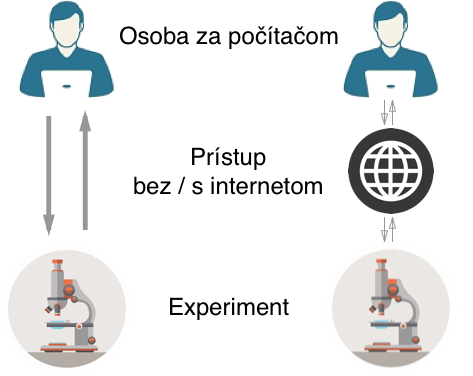
\includegraphics[scale=0.40]{img/VL_vs_real.png}
  \caption{Rozdiel medzi osobne a vzdialene riadneným experimentom.}
  \label{img-real-vs-remote}
\end{figure}

Typický príklad je simulácia experimentu, kde je študent v interakcii s naprogramovaným rozhraním. Ďalšia možnosť je diaľkovo ovládaný experiment, kde študent je v interakcii s reálnym zariadením cez počítačové rozhranie, napriek tomu že sa nenachádza pri ňom. 
Keď vylúčime druhú variantu, tak si môžme utvoriť definíciu nasledovne: \textit{"Virtuálnym laboratóriom voláme to, keď je študent v interakcii s experimentom, ktorý je od neho fyzicky vzdialený alebo nemá na pozadí žiadnu fyzickú realitu"} \cite{hatherly}.\\

Po vysvetlení, čo je VL sa pozrieme na výhody, ktoré nám môže priniesť. Sú popísané v bodoch v tabuľke \ref{table-real-remote-virtual-laboratory}.
Človek často počíta medzi výhody to, že môže nahradiť fyzické laboratórium. Lenže to medzi výhody nepatrí. Nie je možné nahradiť skúsenosti z fyzickej práce so zariadením VL aj keď je to lepšie ako žiadna skúsenosť. VL by nemalo byť vnímané tak, že poskytuje maximálnu možnú skúsenosť.\\

\begin{table}[H]
\small
\begin{tabular}{l l l}
\hline
\textbf{Typ laboratória} & \textbf{Výhody}  & \textbf{Nevýhody} \\ \hline
\textbf{Fyzické} & realistické dáta & obmedzenia na čase a mieste \\
& interakcia s reálnym zariadením & potrebné plánovanie prístupu\\
& lepšia spolupráca & nákladnosť experimentu \\
& interakcia s lektorom & potrebný lektor \\ \hline
\textbf{Virtuálne} & dobré pre vysvetlenie konceptu &  idealizované dáta\\
& bez obmedzenia na čas a miesto &  nedostatok spolupráce  \\
& interaktívne médium & bez interakcie s reálnym zariadením \\
& nízke náklady & \\ \hline
\textbf{Vzdialené} & interakcia s reálnym zariadením &  "virtuálna" prítomnosť v laboratóriu \\
& kalibrácia & \\
& realistické dáta & \\
& bez obmedzenia na čas a miesto & \\
& stredné náklady & \\ \hline
\end{tabular}
\caption{Porovnanie fyzických, virtuálnych a vzdialených a laboratórií.}
\label{table-real-remote-virtual-laboratory}
\end{table}

\subsection{Prehľad existujúcich virtuálnych laboratórií}
V čase písania tohto dokumentu existuje množstvo rôznych virtuálnych/vzdialených laboratórií, ktoré sú používané zahraničnými školami pre výučbu alebo výskum. V práci je zoznam veľmi často používaných laboratórií, ktoré sú prístupne cez internet. Porovnanie funkcionality a využitých technológií je možné vidieť v tabuľke \ref{table-vlab-comparison} \cite{vlabtablecomparison}.

\begin{table}[H]
\scriptsize
\begin{tabular}{l l l l}
\hline\hline
\textbf{Názov} & \textbf{Klient} & \textbf{Server} & \textbf{Prevedenie}\\ \hline
Weblab-DEUSTO & AJAX, Flash, Java applets, & Web services, Python, LabVIEW, & Xilinx-VHDL, LabView\\
&LabVIEW, Remote panel & Java, .NET, C, C++ &\\ \hline
NCSLab & AJAX, Flash & PHP & Matlab, Simulink\\ \hline
ACT & HTML, Java Applets & PHP & Matlab, Simulink\\ \hline
LabShare Sahara & AJAX, Java applets & Web services, Java & Java\\ \hline
iLab & HTML, ActiveX, Java applets & Web services, .NET & LabVIEW\\ \hline
RECOLAB & HTML & PHP & Matlab, Simulink\\ \hline
SLD & AJAX, HTML & Web services, PHP & Matlab, Simulink\\ \hline\hline
\end{tabular}
\caption{Porovnanie virtuálnych laboratórií vytvorených mimo FEI STU.}
\label{table-vlab-comparison}
\end{table}

Následne som preskúmal možnosti existujúcich riešení a vložil do tabuľky \ref{table-feistu}, ktoré boli vytvorené na Fakulte elektrotechniky a informatiky STU \cite{table-vlab-farkas}\cite{table-vlab-borka}\cite{table-vlab-kundrat}\cite{table-vlab-cerveny}\cite{table-vlab-varga}.

\begin{table}[H]
\tiny
\begin{tabular}{l l l l l l}
\hline\hline
\textbf{Rok vypracovania}  & \textbf{Autor} & \textbf{Prevedenie} & \textbf{Spôsob komunikácie} & \textbf{Klient} & \textbf{Server}\\ \hline
2011 &  Roman FARKAŠ & Matlab & JMI, sockets & Java & Java\\
&& Simulink &&& \\
&& Reálna sústava &&& \\ \hline
2012 &  Tibor BORKA  & Matlab & WCF & .NET, WPF & .NET\\
&& Simulink &&& \\
&& Reálna sústava &&& \\ \hline
2014 &  Michal KUNDRÁT  & Matlab & JMI, SOAP & HTML, JS & Tomcat, Java, \\
&& Simulink &&& JSF, EJB3\\ 
&&&&& MySQL\\ \hline
2014 &  Tomáš ČERVENÝ  & Matlab & JMI, HTTP & Mobilné HTML, JS & Jetty, Java\\
&& Simulink &&& \\ \hline
2015 &  Štefan VARGA  & Matlab & COM, HTTP & HTML, JS & PHP, .NET\\
&& Simulink &&& \\ \hline\hline
\end{tabular}
\caption{Porovnanie virtuálnych laboratórií vytvorených na FEI STU.}
\label{table-feistu}
\end{table}

\subsubsection{Nevýhody existujúcich riešení}
Pri tvorbe softwarového systému, či už všeobecne, alebo v našom prípade virtuálneho laboratória je vhodné preskúmať na začiatku možnosti existujúcich riešení. Robí sa to z dôvodu vyvarovania rôznym chybám, ktoré môžu nastať pri návrhu, prípadne overenie technológií, ktoré boli použité a časom už zastarali. V súčasnosti je vývoj nových technológií neskutočne rýchly. Takúto analýzu existujúch riešení sme urobili v predchádzajúcej sekcii.
Naša téma je zameraná na vytvorenie multiplatformového riešenia, kde nie je možné využiť WCF ani COM technológie ako v predchádzajúcich riešeniach. JMI je zase vhodné len pre riešenie, kde sa využíva Java. Pre server nie je možné využiť technológie LabVIEW, .NET (momentálne je už vo vývoji multiplatformová verzia). Čo sa týka klienských riešení tak Flash, ActiveX, Java applets už nie sú podporované v prehliadačoch, taktiež ich nie je vhodné použiť.

\subsection{Komponenty virtuálneho laboratória}
Počet existujúcich laboratórií je veľký, ale väčšinou nie je možné zaručiť kompatibilitu, pretože tu neexistuje žiadny štandard. Každopádne vždy je možné identifikovať základné komponenty, ktoré VL využívajú. Niektoré z nich môžu byť dokonca využité viac krát \cite{article-components-vl}.\\

\noindent Komponenty:
\begin{itemize}
  \item samotný experiment,
  \item zariadenie umožnujúce kontrolu experimentu a získavanie hodnôt,
  \item laboratórny server, ktorý zabezpečí kontrolu, monitorovanie a spracovanie dát z experimentu,
  \item server, ktorý zabezpečí prepojenie medzi vzdialenými užívateľmi a laboratórneho servera, zvyčajne prostredníctvom internetu,
  \item webová kamera pripojená k serveru, ktorá môže byť použitá pre vzdialeného používateľa ako vizuálna a zvuková spätná väzba o stave experimentu,
  \item nástroje umožňujúce viacužívateľské audio, video a chat komunikáciu,
  \item klientský software, pripojiteľný k experimentu.\\
\end{itemize}

Dôležité je uvedomiť si, ktoré z týchto komponentov chceme využiť, pretože na vytvorenie laboratória nie vždy potrebujeme všetky. Prípadne môžeme využiť aj iné, ktoré sa nám dokonale hodia na určitú úlohu. Niekedy sa používa napr. aj databázový server ak chceme experimenty ukladať a spracovávať neskôr. Tak isto je potrebné uvedomiť si, aký typ VL chceme vytvoriť. Určite budú rozdiely pri návrhu jednoužívateľského VL na rozdiel od viacužívateľského, dokonca s viacerými experimentami súčasne. Treba myslieť na to, ako vhodne vyriešiť škálovateľnosť, možné problémy s bezpečnosťou, viacužívateľský prístup, ostatné problémy prístupnosti a podobne.


\section{Použíté technológie}\label{used-technologies}
V predchádzajúcich kapitolách sme popísali ciele, ktoré chceme dosiahnuť. Ďalej sme analyzovali možnosti virtuálnych laboratórií a porovnali ich s už existujúcimi riešeniami. V tejto sekcii budú rozpísané použité technológie. Je samozrejmé, že nie je možné ku každej popísať všetky jej možnosti, ale budeme sa venovať hlavne tým, ktoré plánujeme využiť aj v implementácií.

\subsection{MATLAB R2015b}
Milióny inžinierov a vedcov na celom svete používajú MATLAB na analýzu a návrh systémov a produktov, ktoré menia náš svet. Matlab sa používa v automobilových systémoch, vesmírnych staniciach, smart sieťach, mobilých sieťach LTE alebo aj v škole pri štúdiu. Ďalej sa používa v strojovom učení, spracovaní signálu, spracovaní obrazu, počítačovom videní, komunikácii, finančníctve, riadenií, robotike a existuje množstvo ďalších využití.

Celá platforma Matlab je optimalizovaná pre riešenie inžinierskych a vedeckých problémov. Jazyk Matlab je založený na práci s maticami. Je považovaný za najprirodzenejší spôsob ako počítať matematické úlohy. Pomocou integrovanej grafickej knižnici je možné vizualizovať získáné výsledky z dát. Matlab integruje aj množstvo toolboxov, ktoré pomáhajú priamo začať s algoritmami, ktoré potrebujeme pre našu doménu \cite{matlab-mathworks}.

\subsubsection{Simulink}
Matlab obsahuje viacero integrovaných nástrojov a jeden z nich je aj Simulink. Je to grafické rozhranie, v ktorom je možné modelovať, simulovať a potom aj analyzovať dynamické systémy. Jeho hlavné rozhranie je grafické plátno, spájame jednotlivé bloky do diagramu. Simulink vie úzko spolupracovať s Matlabom, dokonca môže byť z neho skriptovaný, resp. počiatočná inicializácia hodnôt. Matlab a Simulink sú vlastne dve prostredia integrované do jedného softvéru. Čiže je možné simulovať a analyzovať náš model v každom kroku simulácie v oboch prostrediach. Simulink väčšinou spúštame priamo z Matlabu.

\subsubsection{Komunikácia medzi Matlabom a Node.js}
Simulácia dynamickej sústavy, ktorá sa spustí v Simulinku môže odosielať výsledné dáta do Matlab workspace. Odtiaľ ich budeme chciet posielať do Node.js na ďalšie spracovanie. V Matlabe existuje viacero možností získania dát z workspace.\\

\textbf{COM} je prvá z technologických možností. COM bolo vytvorené spoločnosťou Microsoft, teda problémom tohto riešenia je obmedzenie iba na Windows platformu. Používajú sa na prepojenie viacerých aplikácií podporujúcich túto technológiu. Tieto objekty môžu byť vytvorené pomocou rôznych programovacích jazykov, ako napr. C++ alebo Java \cite{matlab-microsoft-com}.
Kým idea COM je celkom jasná, terminológia až toľko nie je.

\verb|COM object| je softwarový komponent, ktorý zodpovedá Component Object Model. COM vnucuje zapuzdrenie objektu a tým predchádza pred priamym prístupom do dát a implementácie. COM objekt poskytne rozhranie, ktoré obsahuje premenné, metódy a udalosti.

\verb|COM client| je program, ktorý používa COM objekty. COM objekty poskytujúce funkcionalitu pre použitie sú volané COM server.

\verb|COM server| môže byť in-process alebo out-of-process. Príklad out-of-process servera je napríklad Microsoft Excel. Microsoft ActiveX control je typu in-process, ktorý vyžaduje kontainer. ActiveX zvyčajne poskytuje užívateľské rozhranie. Príkladom môže byť Microsoft Calendar control. Control container je aplikácia schopná poskytovať ActiveX prvky. Matlab figure okno alebo Simulink model sú tiež príklady control kontajnerov. Matlab može byť použitý ako COM klient aj ako COM automation server \cite{matlab-com}.\\

\textbf{WebSockets} je protokol poskytujúci obojsmernú komunikáciu cez jediné TCP spojenie. WebSoket bol vytvorený a použitý pre webové prehliadače a servery, ale môže byť použitý akýmkoľvek klientom alebo serverom. Špecifikácia protokolu definuje \verb|ws| a \verb|wss| ako nové URI schémy, ktoré sú použité pre nešifrované a šifrované spojenie.

Nevýhodou tohto riešenia pre náš systém je ten, že nie je priamo implementovaný v Matlabe. Keďže pod Matlabom beží JVM, tak je možné implementovať WebSokety pomocou programovacieho jazyku Java a spraviť z toho knižnicu pre Matlab.

Narazili sme na jednu knižnicu vytvorenú týmto spôsobom na odkaze\\ \textit{https://bitbucket.org/kvasnica/wsclient/wiki/Home}. Jej nevýhodou je, že by bolo potrebné inštalovať externé závislosti, ktoré by sa mohli stať nekompatibilné pri zmene Matlabu na vyššiu verziu. Najprv je potrebný \verb|tbxmanager|, ako manažér balíkov a následne pomocou neho inštalácia už konkrétnych balíkov \verb|wsclient, matwebsocks, eventcollector|.\\

\textbf{RESTful web service} patrí medzi modernejšie možnosti komunikácie Matlabu s vonkajším svetom rovnako ako WebSockets. REST je softwarový architektonický štýl, pomocou ktorého vieme posielať a získavať dáta zo serveru. REST komunikuje pomocou HTTP/HTTPS protokolu a zväčša sa používa na CRUD aplikácie, čiže tam kde chceme robiť CREATE, READ, UPDATE, DELETE operácie. Dáta je možné vymieňať medzi klientom a serverom cez \verb|JSON| alebo \verb|XML| správ. Pre jednoduchšie projekty sa používajú viac JSON, hlavne ak sa majú spracovávať JavaScriptom. Výhodou RESTful v tomto riešení je to, že je priamo implementovaný v Matlabe a nie je potrebné inštalovať ďalšie knižnice a toolboxy.

\begin{figure}[H]
  \centering
  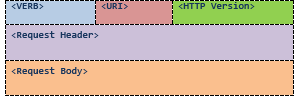
\includegraphics[scale=0.7]{img/rest/rest-http.png}
  \caption{HTTP request.}
  \label{rest-http}
\end{figure}

Na obrázku \ref{rest-http} je štruktúra HTTP requestu. V položke \verb|<VERB>| sa nachádza jedna z HTTP metód GET, PUT, POST, DELETE, OPTIONS, ...

\verb|<URI>| slúži na určenie zdroju, nad ktorým sa bude vykonávať operácia a je tam uložený jeho odkaz.

\verb|<HTTP version>| je verzia HTTP, vo všeobecnosti to bude "HTTP v1.1", ale v novších systémoch môže byť aj "HTTP v2.0".

\verb|<Request Header>| obsahuje metadáta v hlavičke ako kolekciu párov  "key":"value". Tieto nastavenia obsahujú informáciu o správe a jej odosielateľovi ako typ klienta, aký formát podporuje klient, formát správy tela, nastavenia vyrovnávacej pamäte pre odpoveď a mnohé ďalšie informácie.

\verb|<Request Body>| je aktuálny obsah správy. V RESTful službách je toto miesto, kde sa nachádza obsah správy, ktorý sa vymieňa medzi klientom a serverom. V tejto časti nie sú žiadne tagy ani značky pre učenie začiatku alebo konca správy \cite{rest-vaqqas}.

V ukážke POST requestu na obrázku \ref{post-http} zasielame serveru JSON s jednoduchým párom.

\begin{figure}[H]
  \centering
  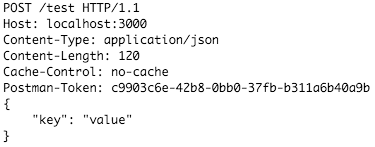
\includegraphics[scale=0.7]{img/rest/post-request.png}
  \caption{HTTP POST request.}
  \label{post-http}
\end{figure}

A zase na obrázku \ref{get-http} v prípade GET requestu vidíme, že získa zdroje, ktoré vracia server, alebo v našom prípade celý obsah HTML stránky, na ktorú bola požiadavka vytvorená.

\begin{figure}[H]
  \centering
  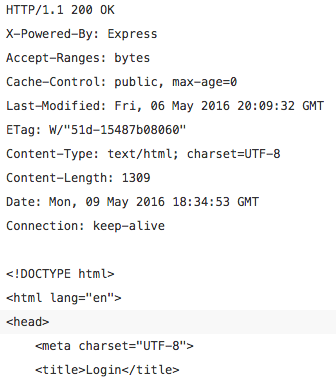
\includegraphics[scale=0.7]{img/rest/get-request.png}
  \caption{HTTP GET request.}
  \label{get-http}
\end{figure}

Teraz, keď sme si vysvetlili v stručnosti ako fungujú RESTful služby, tak sa dostávame k tomu, ako ich je možné využiť v Matlabe. Matlab poskytuje viacero funkcií na prácu s REST ako \verb|weboptions, webread, webwrite.|

Objekt \verb|weboptions| slúži na špecifikáciu parametrov pre RESTful službu. V Matlabe sa volá príkazom \verb|options = weboptions| alebo \verb|options = weboptions(Name,Value)| pričom \verb|Name| je názov parametra, ktorý chceme nastaviť a \verb|Value| jeho hodnota. Je možné nastaviť tieto parametre: \verb|CharacterEncoding, UserAgent, Timeout, Username,| \\ \verb|Password, KeyName, KeyValue, ContentType, ContentReader, MediaType,| \\ \verb|RequestMethod, ArrayFormat|. Ak chceme zobraziť heslo v objekte weboptions, tak na pozícii hesla síce budú hviezdičky, každopádne objekt ukladá heslo ako čistý text. V prípade, keď zavoláme túto vlastnosť v Matlabe cez \verb|options.Password| tak heslo bude viditeľné \cite{matlab-weboptions}.

Objekt \verb|webread| číta obsah z REST služby, na ktorú sme mu poskytli URL cestu a vráti obsah ako štruktúru do požadovanej premennej. Existujú tri najpoužívanejšie možnosti použitia. \verb|data = webread(url)|, kde parameter url je reťazec, v ktorom sa nachádza odkaz na REST službu. \verb|data = webread(url, QueryName1, QueryValue1,| \\ \verb|..., QueryNameN, QueryValueN)|, kde vložené parametre pridá do url volania. Posledná možnosť je \verb|data = webread(___, options)|, kde je môžné špecifikovať posledný objekt ako \verb|weboptions| \cite{matlab-webread}.

A posledný objekt \verb|webwrite|. Tak ako v predchádzajúcom prípade obsahuje zhodné metódy s parametrami, len využitie funkcie je iné. \verb|response = webwrite(url,|\\ \verb|PostName1, PostValue1, ..., PostNameN, PostValueN)| zapíše obsah na špecifikovanú url a vráti response. \verb|response = webwrite(url, data)| zapíše obsah na špecifikovanú url a vráti response. Vstupný parameter data špecifikuje obsah, ktorý je uložený ako pole.\\
\verb|response = webwrite(___, options)| nastaví \verb|weboptions| objekt, zapíše obsah na špecifikovanú url a vráti response.

\subsection{Node.js}
Na stránke platformy \textit{(http://www.nodejs.org)} je Node definovaný ako "platforma založená na JavaScript runtime, ktorý sa nachádza v Chrome pre jednoduchú tvorbu rýchlych a škálovateľných sieťových aplikácií. Node.js používa udalosťami riadený, neblokujúci I/O model, ktorý ho robí nenáročný a efektívny, perfektný pre real-time aplikácie." V súčasnosti patrí medzi najpopulárnejšie JavaScript technológie.

Vďaka jeho súčasnej stabilite ho používa v produkcii mnoho svetových firiem, napríklad eBay, GoDaddy, Microsoft, PayPal, Uber, Yahoo...


\subsubsection{História}
Vytvoril ho Ryan Dahl v roku 2009 a bol dostupný iba pre Linux. Vývoj a údržba bola vedená jeho zakladateľom a neskôr sponzorovaná firmou Joyent. Node.js sa skladá z JavaScriptového engine V8 od Google, udalostnej slučky a nízkoúrovňového I/O API. V roku 2011 bol vytvorený správca balíkov pre Node.js zvaný NPM. Umožnuje programátorom publikovať a zdielať zdrojový kód modulov. Bol navrhnutý tak, aby zjednodušil inštaláciu, aktualizáciu a odinštaláciu modulov. Neskôr v júni 2011, Microsoft a Joyent spolupracovali na implementáci natívnej verzii Node.js pre Windows. V roku 2014 vznikli nezhody pri vývoji, tak programátor Fedor Indutny spravil fork Node.js a vytvoril io.js. Na rozdiel od Node.js autorov, chcel udržiavať io.js aktuálny súčasne s poslednou verziou V8 JavaScript enginu.

Po dohode bola vytvorená Node.js Foundation, ktorá zastrešila vývoj, a spojila Node.js v0.12 a io.js v3.3 do Node.js 4.0, aby znovu spojila roztrieštenú komunitu. Táto verzia priniesla ES6 novinky z V8 do Node.js a súčasne bola vytvorená aj LTS verzia vhodná pre produkčné nasadenie, ktorá ma dlhší vývojový cyklus a príjma len opravy chýb \cite{nodejs-wiki}.

\subsubsection{Architektúra}
Tak ako pri iných platformách aj Node.js má svoju architektúru a v tejto sekcii si popišeme jeho kľúčové vlastnosti. Síce ich nebudeme priamo používať, ale je dobré o nich vedieť.

Má \textbf{asynchrónne a udalosťami riadené} API, čo znamená, že neblokuje vykonávanie nasledujúcich volaní. V podstate ide o to, že server založený na Node.js nikdy nečaká, kým volaná služba/funkcia vráti dáta. Server sa presunie na ďalšie volanie a pomocou notifikačného mechanizmu udalostí získa odpoveď z prechádzajúceho volania, keď bude ukončené a vyzdvihne jeho výsledok.

Vďaka udalostnej slučke je \textbf{jednovláknový a vysoko škálovateľný}. Udalostný mechanizmus pomôže serveru vrátiť odpoveď tak, aby nebol blokovaný a tak robí server vysoko škálovateľný oproti tradičným serverovým riešeniam, ktoré vytvárajú limitovaný počet vlákien na spracovávanie požiadaviek. Node.js spustí jednovláknový program, ktorý môže poskytnúť službu omnoho väčšiemu počtu požiadaviek ako tradičný server Apache httpd. 

Aplikácie sú \textbf{bez vyrovnávajúcej pamäte}, čiže jednoducho posielajú údaje na výstup v malých blokoch.\\

Ako sme už spomenuli, tak platforma Node.js sa skladá z viacerých častí. Bolo by možné ju rozdeliť ešte na menšie časti, ale z nášho pohľadu stačí pre ilustráciu zobrazenie na obrázku \ref{img-node-arch}.

\begin{figure}[H]
  \centering
  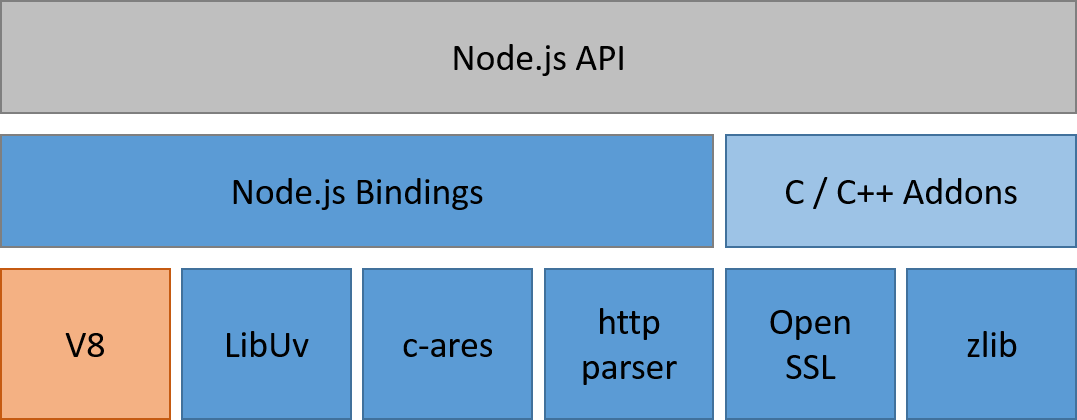
\includegraphics[scale=0.7]{img/node/nodejs-arch.png}
  \caption{Architektúra Node.js platformy.}
  \label{img-node-arch}
\end{figure}

Na vrchole obrázku máme základné Node.js API. Je napísané v JavaScripte a je priamo dostupné programátorom, pre využitie v ich aplikáciach. Pod týmto základným API je knižnica, ktorá viaže C/C++ s JavaScriptom. Node.js tiež poskytuje doplnky (addons), čo sú dynamicky linkované zdielané objekty. Tie sa viažu na C/C++ knižnice. To znamená, že môžeme využiť skoro akúkoľvek C/C++ knižnicu a vytvoriť z nej doplnok, ktorý je použiteľný v Node.js.\\

\noindent Pod týmto všetkým máme už len natívne knižnice vytvorené v C/C++:

\textbf{V8} je open source JavaScript engine, ktorý bol vytvorený pre internetový prehliadač Google Chrome. Je napísaný v C++ a je možné ho spustiť samostatne alebo v ktorejkoľvek C++ aplikácií. V podstate kompiluje JavaScript kód do natívneho strojového kódu, namiesto toho, aby bol interpretovaný.

\textbf{Libuv} je multiplatformová podporná knižnica so zameraním na asynchónne I/O operácie. Zo začiatku Node.js začal používať \verb|libuv| ako abstrakčnú vrstvu pre \verb|libev| a \verb|libio|, ale neskôr sa libuv stala robustnejšia a nahradila túto funkcionalitu, aby sa mohla stať multiplatformovou. Keď V8 spravuje vykonávanie JavaScriptu, tak libuv spravuje udalostnú slučku (event loop) a asynchrónne I/O operácie. V tomto zozname sú všetky možnosti \verb|libuv|:
\begin{itemize}
\item plnohodnotná údalostná slučka, ktorú tvorí epoll, kqueue, IOCP a udalostné porty,
\item asynchrónne TCP a UDP sokety,
\item asynchrónne DNS,
\item asynchrónne operácie nad súbormi a súborovým systémom,
\item udalosti nad súborovým systémom,
\item preklad ANSI kódov kontrolovaných cez TTY,
\item IPC so zdielaním soketu s využitím Unix soketov alebo pomenované kanály (vo Windows),
\item detské procesy,
\item vlákna a synchronizácia,
\item riadenie signálov,
\item hodiny s presným časovaním (hight resolution clock).
\end{itemize}

\textbf{c-ares} je C knižnica pre asynchrónne DNS žiadosti vrátane prekladania názvov. Je určená pre aplikácie, ktoré potrebujú vykonávať dotazy na DNS bez blokovania, alebo ak potrebujú vykonať niekoľko dotazov paralerne.

\textbf{http\_parser} je parser pre požiadavky a odpovede HTTP napísaný v C. Nerobí žiadne systémové volania ani alokácie, neukladá dáta do vyrovnávacej pamäte a môže byť zrušený okamžite. Jeho hlavné vlastnosti sú:
\begin{itemize}
\item nemá žiadne závislosti,
\item udržiava trvalý stream
\item dekódovanie blokového kódovania,
\item chráni buffer proti útokom.
\end{itemize}

\textbf{OpenSSL} je open source implementácia SSL v2/v3 a TLS v1 protokolov ako aj kryptografická knižnica pre všeobecné účely. Je založená na SSLeay knižnici. Tá poskytuje všetky potrebné kryptografické metódy ako je hash, hmac, cipher, decipher, sign a verify metódy.

\textbf{Zlib} je všeobecná knižnica na kompresiu dát napísaná v C \cite{nodejs-arch}.


\subsubsection{Event loop}
Udalostná slučka (event loop) dáva Node.js možnosť zvládnuť veľké množstvo súčasných požiadaviek aj keď je spustený v "jednom vlákne". V každej udalostne riadenej aplikácií je vo všeobecnosti hlavná slučka, ktorá počúva a čaká na udalosti a keď udalosť je zaregistrovaná, tak sa zavolá callback funkcia. Na obrázku \ref{img-node-event-loop} je zjednodušený pohľad na to, ako to funguje vrámci Node.js.

\begin{figure}[H]
  \centering
  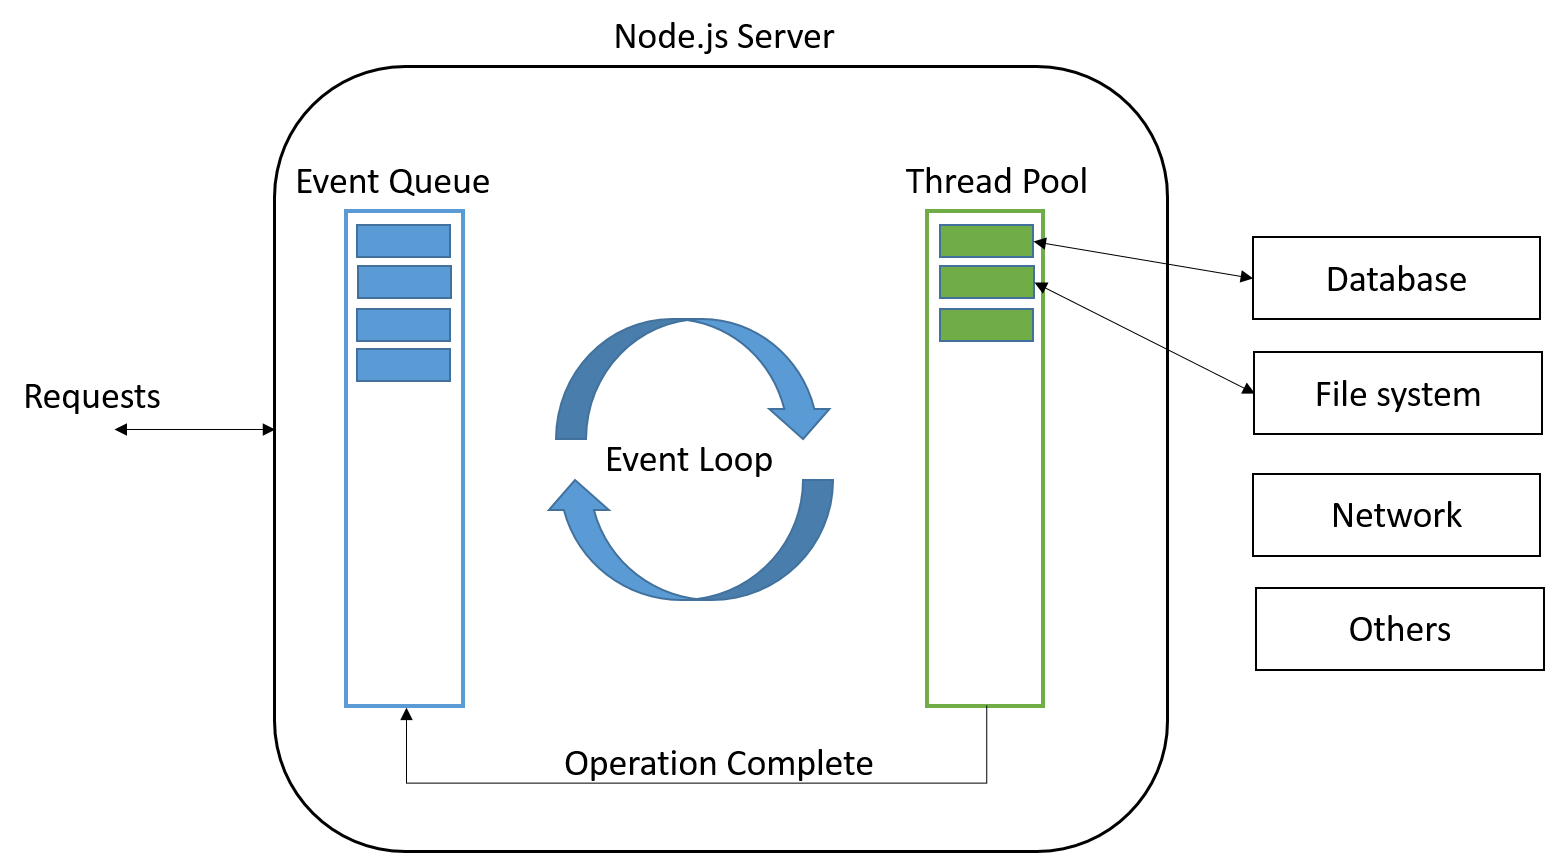
\includegraphics[scale=0.58]{img/node/nodejs-event-loop.png}
  \caption{Udalostná slučka v Node.js.}
  \label{img-node-event-loop}
\end{figure}

Udalostná slučka jednoducho prechádza cez frontu, čo je vlastne zoznam udalostí a callbackov vykonaných operácií. Všetky I/O operácie sú vykonané asynchrónne vláknami vo "vláknovom stacku" (thread pool). Tu zohráva dôležitú úlohu libuv. Ak nejaká položka vyžaduje I/O operáciu, tak udalostná slučka jednoducho prenechá operáciu vláknovému stacku. Udalostná slučka pokračuje vo vykonávaní položiek v udalostnej fronte. Keď je I/O operácia hotová, tak callback je zaradený na spracovanie. Udalostná slučka vykoná callback a poskytne požadované výstupy. A takto sa celý proces opakuje \cite{nodejs-event-loop}.

\subsubsection{Možnosti a využitie}
Na základe popísaných základných častí Node.js v predchádzajúcich sekciách si ukážeme možnosti využitia, resp. výhody a nevýhody \cite{nodejs-arch}.\\

\noindent \textbf{Výhody}
\begin{itemize}
\item asynchrónne I/O - vhodné pre webové a sieťové aplikácie,
\item rôzne možnosti škálovania,
\item programovací jazyk je JavaScript, čiže rovnaký jazyk pre backend aj frontend aplikácie,
\item rýchly prechod od Javy, .NET stačí len zmeniť myslienie na asynchrónne,
\item veľmi aktívna komunita, ktorá zdieľa množstvo kódu na verejných repozitároch ako github,
\item rýchlo rastúca NPM komunita s množstvom modulov pripravených na použitie.
\end{itemize}

\noindent \textbf{Nevýhody}
\begin{itemize}
\item veľmi neefektívne pre úlohy náročné na CPU, ako generovanie reportov, analýzy, výpočty...
\item použitím udalosťami riadenej metodológie bez pochopenia prístupu môže viesť k nevhodne napísaným kódom (napr. "callback hell"),
\item neexistuje toľko štandardných knižníc ako pri Java, .NET platforme ako sú napr. XML parsery, alebo zložitejšie dátové štruktúry.
\end{itemize}

Ako teda vidíme, Node.js nie je vhodný na všetky úlohy, ale vždy záleží od konkrétnej potreby. Čiže ak potrebujeme streaming alebo rýchly upload súborov, real-time získavanie údajov, single page aplikácie, websokety, tak je na takéto úlohy veľmi vhodný. Vo všeobecnosti všade kde sa používajú I/O operácie, tak vie zvládnuť veľké množstvo súčasných spojení \cite{nodejs-introduction}.

\subsection{Node Package Manager}
Node.js po nainštalovaní obsahuje aj \verb|NPM|. NPM je program, ktorý sa spúšta z príkazového riadku, pomocou ktorého vieme sťahovať moduly z centrálneho repozitára\\ \textit{https://www.npmjs.org}. Rovnako je možné vytvoriť aj vlastný modul a uložiť ho do repozitára.

Každý modul by mal mať vlastný adresár, ktorý tiež obsahuje súbor s metadátami volaný \verb|package.json|. V tomto súbore musia byť nastavené vlastnosti a ich hodnoty ako na obrázku \ref{img-npm-packagejson}, čiže: \verb|name| a \verb|version| \cite{nodejs-by-example}.

\begin{figure}[H]
  \centering
  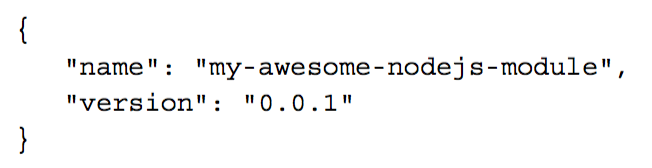
\includegraphics[scale=0.7]{img/npm/npm-minimum.png}
  \caption{Potrebné vlastnosti nastavené v package.json.}
  \label{img-npm-packagejson}
\end{figure}

Ďalšia dôležitá vec je, že pri \verb|version| musíme používať sémantické verziovanie\\ (\textit{http://semver.org/}), kde pri verzií \verb|1.2.3| je prvá major verzia, druhá minor a tretia len oprava chýb.

\subsubsection{Použitie modulov}
Vo všeobecnosti existujú tri možnosti ako použiť moduly, ktoré sú už publikované na npmjs.org. Všetky tri možnosti si vyžadujú použitie Node manažéra na prácu s balíkmi: \cite{nodejs-by-example}

\begin{itemize}
\item môžme nainštalovať špecifický modul manuálne tak, že sa presunieme do požadovaného priečinka a zavoláme v termináli \verb|npm install nazov-modulu|. Správca balíkov nainštaluje poslednú verziu modulu a vloží ju do priečinka \verb|node_modules|. V prípade použitia, nevoláme celú cestu, ale len \verb|require(nazov-modulu)|.
\item inštalácia modulu globálne pre celý systém s použitím \verb|-g| prepínača v príkaze. \verb|npm install nazov-modulu -g|. Toto použitie slúži skôr na inštaláciu vývojových nástrojov, ktorých verzia sa tak často nemení a nie na bežné moduly.
\item posledná možnosť je príkaz \verb|npm install| v priečinku, kde sa nachádza už spomínaný súbor \verb|package.json| a má v sebe vlastnosť \verb|dependencies| ako na obrázku \ref{img-npm-dependencies}.
\end{itemize}

\begin{figure}[H]
  \centering
  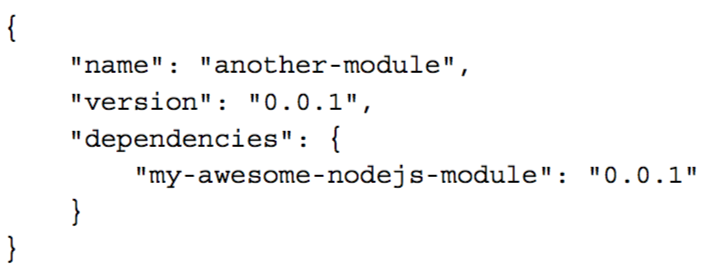
\includegraphics[scale=0.7]{img/npm/npm-overview-dependency.png}
   \caption{Dependencies vlastnosť v package.json.}
  \label{img-npm-dependencies}
\end{figure}

\subsubsection{Vstavané moduly}
Node.js je považovaný za technológiu, pomocou ktorej môžeme programovať serverové aplikácie. Často potrebujeme robiť rôzne úlohy. V Node.js existujú veľmi nápomocné moduly, ktoré môžeme využiť \cite{nodejs-by-example}.

\subsubsection{Vytvorenie web servera pomocou HTTP modulu}
Modul \verb|http| patrí asi medzi najviac používané, pretože vďaka nemu spustíme web server na konkrétnom porte - obrázok \ref{img-npm-http}.

\begin{figure}[H]
  \centering
  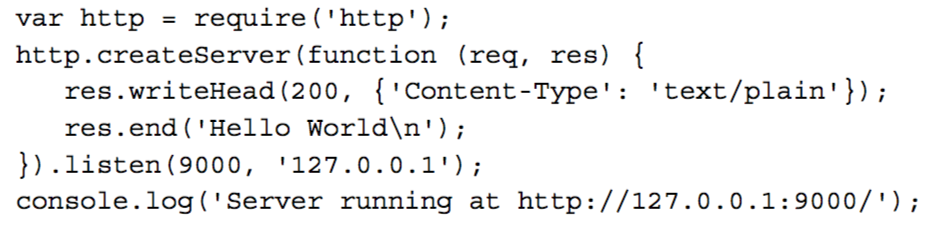
\includegraphics[scale=0.7]{img/npm/npm-http-module.png}
  \caption{Volanie HTTP modulu v Node.js a spustenie servera.}
  \label{img-npm-http}
\end{figure}

Máme dostupnú metódu \verb|createServer()|, ktorá vracia nový web server objekt. Často hneď za tým voláme aj \verb|listen()| metódu pre nastavenie portu. Ak je potrebné tak pomocou funkcie \verb|close()| zastavíme prijímanie nových požiadaviek. Telo callback funkcie, ktorú používame, má vždy \verb|request| a \verb|response| objekty. Prvý objekt sa používa na získanie informácií o prichádzajúcich požiadavkách ako napr. parametre z \verb|GET| a \verb|POST| \cite{nodejs-by-example}.


\subsection{Express.js}
Express.js patrí medzi minimalistické a flexibilné Node.js webové frameworky. Poskytuje robustné možnosti pre vývoj webových a mobilných aplikácií. Uľahčuje vývoj webových aplikácií založených na Node.js \cite{express-tutorial}.\\

\noindent Medzi jeho hlavné možnosti patrí:
\begin{itemize}
\item možnosť nastaviť middleware funkciu pre odpovede na HTTP požiadavky,
\item definuje smerovaciu tabuľku, ktorá je použitá na vykonanie požiadaviek založených na HTTP,
\item umožňuje dynamicky vykreslovať HTML stránky, tak aby bolo možné vkladať argumenty do šablóny.
\end{itemize}

Vo väčšine prípadov web aplikácií s použitím Expressu inštalujeme aj \verb|body-parser|, ktorý slúži ako middleware pre narábanie s JSON, Raw, Text a URL parametrami.

\subsubsection{Web server}
Následujúca ukážka na obrázku \ref{img-express-base} je základná kostra Express aplikácie, ktorá spustí web server a počúva na porte 8081. Po príchode na stránku bude vždy odpovedať textom \textbf{Hello wordl!} \cite{express-tutorial}.

\begin{figure}[H]
  \centering
  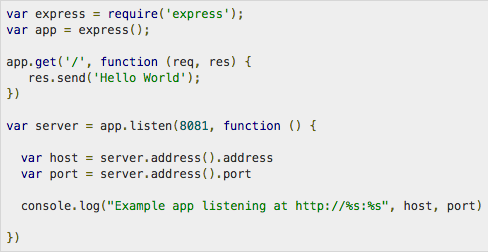
\includegraphics[scale=0.7]{img/express/express-example.png}
  \caption{Spustenie web servera na porte 8081.}
  \label{img-express-base}
\end{figure}

Na spustenie je potrebné vložiť tento kód do súboru s koncovkou app\textbf{.js} a následne spustiť \verb|node app.js|, čoho výsledkom bude výstup v termináli \textbf{Example app listening at http://0.0.0.0:8081}.

\subsubsection{Request a response objekty}
Ak webová aplikácia používa smerovanie, tak obsahuje objekty request a reponse z Node.js, ktoré sú dostupné v callback funkcii. Na obrázku \ref{express-res-req} je smerovanie na hlavnú stránku \cite{express-tutorial}.

\begin{figure}[H]
  \centering
  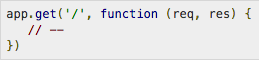
\includegraphics[scale=0.7]{img/express/express-req.png}
  \caption{Objekt req a res ako parametre callback funkcie.}
  \label{express-res-req}
\end{figure}

\textbf{Request} objekt reprezentuje HTTP request a obsahuje isté vlastnosti a funkcie. Ich zoznam je celkom dlhý a nebudeme ich potrebovať všetky. Ale niektoré stoja za zmienku ako \verb|req.body|, obsahujúci páry \verb|"kľúč": "hodnota"|, ktoré sú vytvorené pre telo správy. \verb|req.cookies| umožňuje získať cookies z klienta na server. \verb|req.params| slúži na získanie parametrov z URL, keď používame dynamické volania ako napr. \textbf{/user/:id} tak \textbf{id} je parameter dostupný v \verb|req.params.id|. Čo sa týka funkcií request objektu, tak tie zvyčajne nie sú používané \cite{nodejs-exp-request}.

\textbf{Response} objekt predstavuje HTTP response, ktorý Express odošle po prijatí GET prípadne POST požiadavky. Pri tomto popise nie sú pre nás zaujímavé vlastnosti, ale skôr funkcie. Pomocou \verb|res.cookie(name, value [, options])| vieme nastaviť hodnotu cookie a pomocou \verb|res.clearCookie(name [, options])| ju zase vymazať. Ďalej môžeme odoslať kód, aby klient vedel akým statusom skončila požiadavka. Používa sa na to funkcia \verb|res.status(200).end()|, kde číselný kód sa určuje podľa štandardných HTTP status hodnôt. Užitočná je aj funkcia \verb|res.json({ user: 'xstark' })| pre zaslanie odpovede vo formáte JSON. V prípade, že potrebujeme presmerovanie na inú stránku, tak použijeme funkciu \verb|res.redirect([status,] path)| \cite{nodejs-exp-response}.

\subsubsection{Smerovanie}
Smerovanie (routing) slúži na určenie, ako bude aplikácia reagovať na požiadavku klienta, čo zahŕňa URI a špecifické metódy (GET, POST, PUT, DELETE, ...) HTTP požiadavky \cite{express-tutorial}.
Každý \verb|route| môže mať viacero callback funkcií, ktoré sa vykonajú len ak je zavolané dané smerovanie.\\

\noindent Definícia route má následujúcu štruktúru \verb|app.METHOD(PATH, CALLBACK)|, kde:
\begin{itemize}
\item \verb|app| je inštancia express,
\item \verb|METHOD| je jedna z dostupných HTTP metód,
\item \verb|PATH| je cesta na serveri,
\item \verb|CALLBACK| je funkcia, ktorá sa vykoná v prípade, že sa zhoduje cesta \cite{express-routing}.
\end{itemize}

\subsubsection{Middleware}
Funkcie označované middleware, sú také, ktoré majú prístup do request \verb|(req)|, response \verb|(res)| objektu a následujúcej middleware funkcie. Následujúca funkcia sa bežne označuje názvom \verb|next| \cite{express-middleware}.\\

\noindent Úlohy middleware funkcií:
\begin{itemize}
\item vykonávať akýkoľvek kód,
\item robiť zmeny na \verb|request| a \verb|response| objekoch,
\item ukončiť request-reponse cyklus,
\item zavolať ďalšiu middleware funkciu v poradí. 
\end{itemize}

Obrázok \ref{img-express-middleware} popisuje vlastnosti middleware funkcie. V prípade, že funkcia neukončí volanie, musí posunúť obsluhu ďalšej middleware funkcii zavolaním \verb|next()|. Inak sa request zasekne a klient bude stále čakať na odpoveď kým sa po určitom omeškaní ukončí \cite{express-middleware}.

\begin{figure}[H]
  \centering
  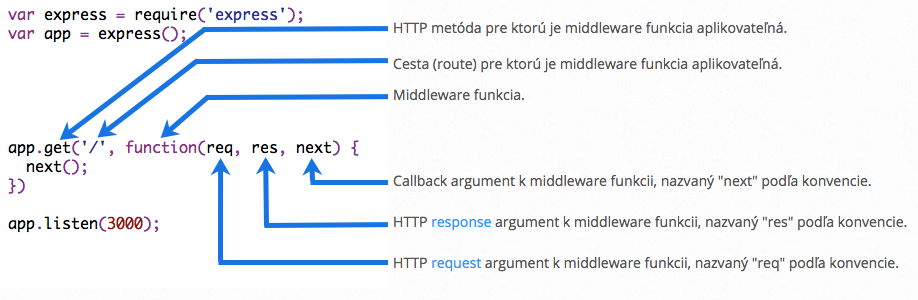
\includegraphics[scale=0.5]{img/express/express-middleware.png}
  \caption{Vlastnosti middleware funkcie \cite{express-middleware}.}
  \label{img-express-middleware}
\end{figure}

\subsection{MongoDB}
MongoDB je multiplatformová dokumentovo orientovaná databáza. Je klasifikovaná ako NoSQL databáza, čo znamená, že nepoužíva klasickú tabuľkovú štruktúru ako v relačnej databáze, ale objekty vo forme JSON dokumentov s dynamickými schémami (v MongoDB sa volá tento formát BSON). Vďaka formáte JSON dokumentov je možné ukladať dáta z rôznych aplikácií rýchlejšie a jednoduchšie \cite{mongodb-wiki}.

Príklad dokumentu, ktorý sa ukladá do MongoDB vidíme na obrázku \ref{mongodb-example}. V jednoduchých prípadoch ako tento nie je vidieť žiadny rozdiel oproti klasickému JSON.

\begin{figure}[H]
  \centering
  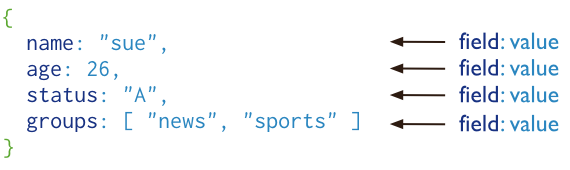
\includegraphics[scale=0.5]{img/mongodb/crud-annotated-document.png}
  \caption{JSON dokument v MondoDB.}
  \label{mongodb-example}
\end{figure}

\subsection{Angular.js}
Angular.js, bežne označovaný aj ako Angular. Je open source framework pre web vytvorený Slovákom Miškom Hevery do verzie 1.0. Neskôr vývoj a údržbu frameworku prevzal Google. Bol vytvorený za účelom tvorby SPA, teda takých webových aplikácii, v ktorých je možné aktualizovať svoj obsah bez toho, aby si užívateľ toho vo väčšej miere všimol. Cieľom je zjednodušiť vývoj, ale aj testovanie klientských webových aplikácií na MVC alebo MVVM architektúre.

Framework funguje tak, že pri prvom načítaní HTML stránky vloží k elementom vlastné atribúty. Angular interpretuje tieto atribúty ako direktívy a viaže ich vstupno-výstupné časti ako model, ktorý je reprezentovaný štandardnými premennými JavaScriptu. Hodnoty týchto premenných môžu byť manuálne nastavené v kóde, alebo získané zo statických (väčšinou uložených na súborovom systéme), dynamických (získaných z RESTful služby) JSON súborov.

Slúži ako klientská súčasť MEAN vývojarského stacku, čo je vlastne \textbf{M}ongoDB databáza, \textbf{E}xpress.js web server framework, \textbf{A}ngular.js  a \textbf{N}ode.js ako web server \cite{angular-wiki}\cite{angular-docs}.

\subsubsection{Koncept}
Angular ako framework sa skladá z viacerých časti, z ktorých každá má svoju úlohu. Na obrázku \ref{img-angular-concept} sú zobrazené základné komponenty, z ktorých sa skladá. Nižšie si popíšeme hlavne tie, ktoré chceme využíť v našom softvérovom riešení \cite{angular-concept}.

\begin{figure}[H]
  \centering
  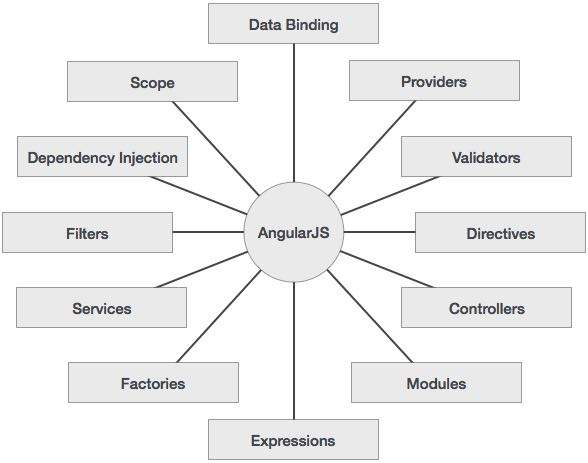
\includegraphics[scale=0.5]{img/angular/angularjs_concepts.jpg}
  \caption{Koncept frameworku Angular.js.}
  \label{img-angular-concept}
\end{figure}

\subsubsection{Direktívy}
V jednoduchosti direktívy sú značky na DOM elemente (napr. atribút, element, komentár alebo CSS trieda), ktorá povie Angular HTML kompilátoru - \verb|$compile|, aby priradil špecifické správanie na daný DOM element (pomocou \textbf{event listenerov}), alebo dokonca transformoval DOM element na svoje dieťa. V šablónach sa spájajú informácie z modelu a kontroleru pre renderovanie dynamického obsahu, ktorý potom vidí užívateľ vo webovom prehliadači.

Angular je dodávaný so vstavanými direktívami, od ktorých sa očakáva, že budú využívané často. Napr. \verb|ng-bind|, \verb|ng-model|, \verb|ng-class| \cite{angular-docs}.

\subsubsection{Scope}
Scope je objekt, ktorý odkazuje na model aplikácie. V tomto kontexte sa vykonávajú výrazy. Scopes sú usporiadané do hierarchickej štruktúry, ktorá napodobňuje DOM štruktúru aplikácie. V scope je možné sledovať model pomocou \verb|$watch| a vykonávať udalosti s \verb|$apply| cez celý systém do zobrazenia. Slúži na previazanie aplikačného kontroleru a zobrazenia. Rovnako ako kontroler aj direktívy majú prístup k scope, ale nie navzájom medzi sebou. Vďaka tomu je kontroler izolovaný od direktívy a tak isto aj od DOM.

Každá aplikácia ma práve jeden \verb|$rootScope|, ale môže mať viacero detských \verb|$scope|. Aplikácia môže mať viacero scopes, pretože niektoré direktívy môžu vytvoriť nový detský scope, ak to potrebujeme. Keď je nový scope vytvorený, tak je priradený ako detský k rodičovskému scope. Tento systém vytvára stromovú štruktúru paralernú k DOM, v ktorej sú vytvorené \cite{angular-docs}.

Často používaná operácia pre zistenie zmien na objekte v scope sa volá \textbf{dirty checking} a preto by mala byť efektívna. V závislosti od potreby môže byť dirty checking využité týmito troma stratégiami: referenciou na objekt, obsah poľa alebo na hodnoty objektu - obrázok \ref{img-angular-watch}.

\begin{figure}[H]
  \centering
  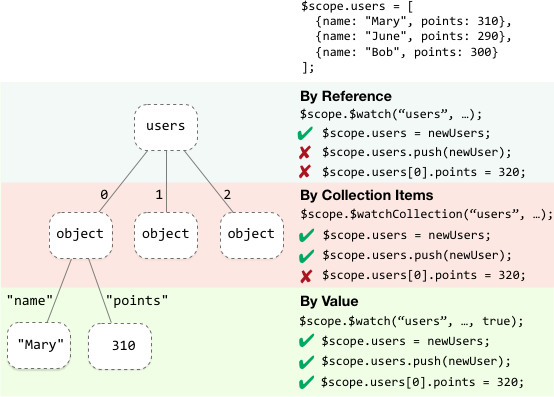
\includegraphics[scale=0.7]{img/angular/concepts-scope-watch-strategies.png}
  \caption{Možnosti sledovania modelu v Angular.js.}
  \label{img-angular-watch}
\end{figure}

\noindent Líšia sa v spôsobe sledovania zmeny a výkonostnými rozdielmi:
\begin{itemize}
  \item \textbf{podľa referencie:} \verb|$scope.$watch(watchExpression, listener)| - detekcia zmeny, keď sa na sledovanú hodnotu nastaví nová. Ak sa zmení vnorený objekt alebo pole objektu ktorý sledujeme, zmeny vnútri nie su detekované. Toto je najrýchlejšia stratégia.
  \item \textbf{na celej kolekcii:} \verb|$scope.$watchCollection(watchExpression, listener)| - detekcia zmien, ku ktorým dochádza vo vnútri poľa alebo objektu. Napr. keď sú položky pridané, odstránené alebo sa v nich zmenilo poradie. Detekcia je plytká, čiže nesleduje vnorené polia. Sledovanie celého obsahu kolekcie je výkonovo náročnejšie ako sledovanie na referenciu, pretože treba uchovávať kópiu obsahu. Avšak, táto stratégia sa snaží minimalizovať množstvo potrebných kopírovaní.
  \item \textbf{všetky položky objektu:} \verb|$scope.$watch(watchExpression, listener, true)| - detekcia akéjkoľvek zmeny v ľubovolnej vnorenej štruktúre. Táto stratégia má najväčšie možnosti detekcie zmien, ale za to je výkonovo aj pamäťovo najnáročnejšia. Je potrebné uchovávať kópiu celej vnorenej štruktúry a pri každej zmene, sa musí skopírovať do pamäte.
\end{itemize}


\subsubsection{Výrazy}
Výrazy (expressions) sú malé časti kódu v JavaScripte umiestnené medzi dvojité zložené zátvorky.

Príklad: \verb|<span title="{{ attrBinding }}">{{ textBinding }}</span>|. Vyhodnotenie môže ale prebehnúť aj vo funkcii na kliknutie \verb|ng-click="functionExpr()"|.
Pre príklad pridávam zopár ďalších platných výrazov, ktoré sa často môžu používať: \verb|{{ 1 + 2 }}, {{ a + b }}, {{ user.name }}, {{ items[index] }}| \cite{angular-docs}.

%\textbf{Compiler}

%\textbf{Filter}

%\textbf{View}


\subsubsection{Previazanie dát}
Data binding v Angulare funguje ako automatická synchronizácia dát medzi modelom a zobrazením. Ak sa zmení model, tak zmena sa automaticky prejaví aj do zobrazenia a naopak.
Na obrázkoch \ref{img-angular-onedb} a \ref{img-angular-twodb} môžeme vidieť rozdiel medzi jednosmerným a obojsmerným data bindingom.

\begin{figure}[H]
\subfigure[Jednosmerný data binding]{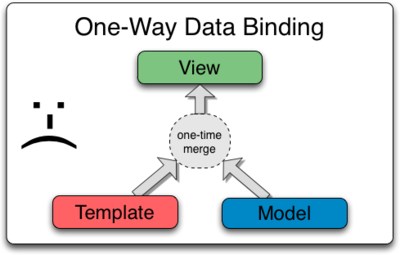
\includegraphics[scale=0.53]{img/angular/One_Way_Data_Binding.png}\label{img-angular-onedb}}
\subfigure[Obojsmerný data binding]{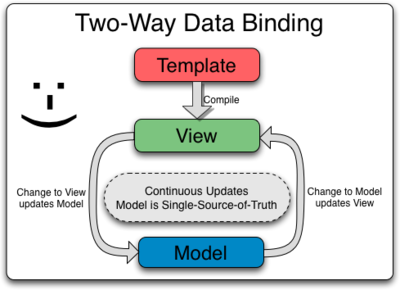
\includegraphics[scale=0.53]{img/angular/Two_Way_Data_Binding.png}\label{img-angular-twodb}}
\caption{Data binding v Angular.js.}
\end{figure}

Mnoho šablónovacích enginov nastavujú dáta len v jednom smere: spoja šablónu a komponenty modelu spolu do zobrazenia. Keď sa dokončí spojenie, zmeny v modeli alebo jeho príslušných sekcií v zobrazení sa neprejavia automaticky. Horšie je, že zmeny ktoré úžívateľ urobí v zobrazení sa neprejavia do modelu. To znamená, že vývojár musí napísať kód, ktorý sústavne synchronizuje zobrazenie s modelom a naopak.

Šablóny v Angulari fungujú inak. Šablóna (čo je neskompilovaný HTML kód spolu s ďalšími značkami a direktívami) je najprv kompilovaná vo webovom prehliadači. Tento krok už produkuje živé zobrazenie. Akékoľvek zmeny v zobrazení sa okamžite prejavia v modeli, a akékoľvek zmeny v modeli sú poslané do zobrazenia. Vďaka tomuto spôsobu môžeme o zobrazení hovoriť ako o okamžitej projekcii modelu.

Pretože zobrazenie je iba projekcia modelu, tak kontroler je kompletne separovaný od zobrazenia a nevedia o sebe. Vďaka tomu je testovanie jednoduchšie, pretože je možné testovať kontroler nezávisle od zobrazenia \cite{angular-docs}.

\subsubsection{Kontroler}
V Angulare je kontroler definovaný funkciou konštruktoru v JavaScripte, ktorý je používaný pre rozšírenie Scope. Keď je kontroler pripojený k DOM cez \verb|ng-controller| direktívu, tak sa vytvorí inštancia objektu konštruktora. Bude vytvorený detský Scope a je dostupný ako parameter do funkcie konštruktora kontroléru ako \verb|$scope|.

Obrázok \ref{img-angular-controller-def} ukazuje spôsob definície kontroleru v JavaScript súbore a jeho následné volanie v HTML šablóne.

\begin{figure}[H]
  \centering
  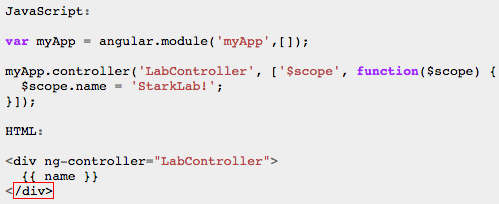
\includegraphics[scale=0.7]{img/code/angular-controller-def.png}
  \caption{Kontroler v Angular.js a jeho volanie na HTML elemente.}
  \label{img-angular-controller-def}
\end{figure}

Vo všeobecnosti by kontroler nemal toho robiť veľa. Mal by obsahovať iba biznis logiku potrebnú pre konkrétne zobrazenie. Najlepší spôsob ako zachovať kontroler čo najmenší, je zabalenie niektorej úlohy do služby (service), ktorá tam nepatrí. Potom tieto úlohy zo služieb voláme v kontroleri ako závislosť \cite{angular-docs}.\\

\noindent Kontroler je možné použiť na:
\begin{itemize}
\item nastavenie počiatočného stavu v \verb|$scope| objekte.
\item pridanie vlastností a správania do \verb|$scope| objektu.\\
\end{itemize}

\noindent Nepoužívať kontroler na:
\begin{itemize}
\item manipuláciu s DOM, pretože kontroler by mal obsahovať iba biznis logiku. Vložením akéjkoľvek prezentačnej logiky do kontroleru vo veľkej miere ovplyvňuje jeho testovanie. Na manipuláciu slúžia direktívy.
\item formátovanie vstupu - použiť angular form controls.
\item filtrovanie výstupu - použiť angular filter.
\item zdielanie kódu alebo stavu naprieč kontrolermi - použiť angular service.
\item správa životného cyklu ostatných komponentov (napr vytváranie inštancií service).
\end{itemize}

%\textbf{Dependency Injection}

\subsubsection{Moduly}
Moduly (module) môžeme rozumieť ako kontainer pre rozličné časti našej aplikácie - \verb|controller|, \verb|service|, \verb|filter|, \verb|directive|... Každý modul môže obsahovať zoznam iných modulov ako svoju závislosť. Keď má modul zavíslosť na inom module, tak tento musí byť načítaný ešte pred našim modulom. Poradie môžeme manuálne nastaviť v konfigurácii modulov. Každý modul môže byť načítaný iba raz aj keď na ňom závisí viac modulov \cite{angular-docs}.

Pri programovaní modulov musíme dávať pozor na to, aby sme si neprepísali už existujúci v pamäti. Postup vytvorenia na obrázku \ref{img-angular-module-def}.

\begin{figure}[H]
  \centering
  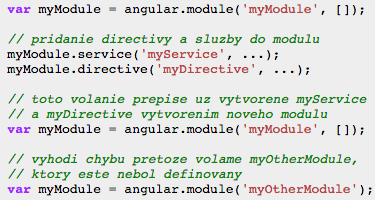
\includegraphics[scale=0.7]{img/code/angular-module.png}
  \caption{Vytvorenie modulov a pridanie ich funkcionality.}
  \label{img-angular-module-def}
\end{figure}

\subsubsection{Služby}
Služby (service) sú nahraditeľné objekty, ktoré je možné použiť v aplikácií pomocou systému závislostí. Používajú sa pre lepšiu organizáciu a zdieľanie kódu naprieč celej aplikácie. Framework poskytuje mnoho užitočných služieb, ako napr. \verb|$http|, ale väčšina aplikácií má potrebu si vytvoriť vlastné \cite{angular-docs}.\\

\noindent Poznáme dva typy služieb:
\begin{itemize}
\item lazily instantiated - angular vytvorí inštanciu služby iba v prípade, že na nej závisí komponent/modul,
\item singleton - každý komponent závisiaci na službe získa referenciu na jedinú inštanciu generovanú zo service factory.
\end{itemize}

%\subsubsection{Scope}
%\subsubsection{Bootstrap aplikácie}
% mozno lepsie pred konceptom
%\subsubsection{Two-way data binding}

\section{Porovnanie platforiem}

V predchádzajúcej sekcii sme si popísali technológie, ktoré plánujeme využiť. Keď si to všetko spojíme dohromady, tak dostaneme základný obraz, ako by mohlo vyzerať naše riešenie na platforme Node.js - obrázok \ref{img-plat-node}. Na následujúcich obrázkoch sme porovnali našu vybranú platformu s inými možnými riešeniami. Tieto riešenia sú tvorené na strane servera (backend) a klientská časť (frontend) je realizovaná pomocou technológie Angular.js v prehliadači.

Základná časť, na ktorej to celé stojí je operačný systém. Ten v tomto prípade môže byť ľubovolný. Nad ním je už spomínaný Node.js, ktorý má v sebe \verb|http| modul. Ten umožnuje vytvorenie jednoduchého a rýchleho webového servera. Tento modul je štandardná súčasť Node.js. Je možné ho vymeniť za iný, ale väčšinou nie je na to dôvod. Ďalej nám umožnuje pripojenie na ľubovolnú databázu pomocou dostupných modulov. Komunikácia medzi Node.js a Matlabom prebieha cez RESTful služby. Posledná časť nášho riešenia je Express.js framework pre uľahčenie práce s Node.js API. Výhoda tohoto riešenia je hlavne použitie jazyka JavaScript pre programovanie na serverovej aj klientskej časti.

\begin{figure}[H]
  \centering
  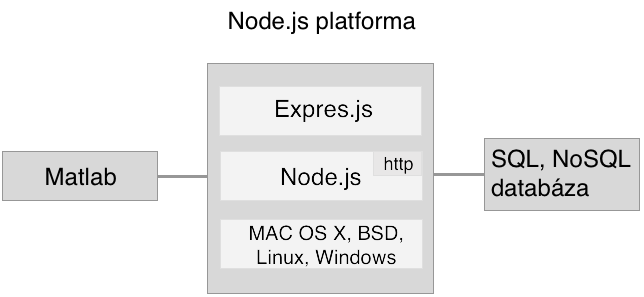
\includegraphics[scale=0.6]{img/platf/node-platform.png}
  \caption{Platforma Node.js.}
  \label{img-plat-node}
\end{figure}

Pre porovnanie tu máme aj WAMP riešenie - obrázok \ref{img-plat-php}, ktorý vyzerá podobne ako Node.js platforma vyššie. Rozdiel je v tom, že PHP je len modul do webového servera Apache httpd. V tomto prípade by bola možnosť vybrať aj iný http server napr Nginx.

\begin{figure}[H]
  \centering
  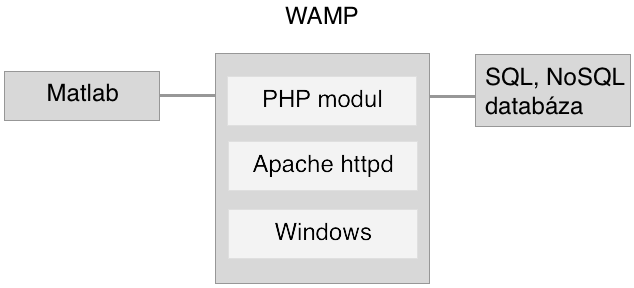
\includegraphics[scale=0.6]{img/platf/php-platform.png}
  \caption{Platforma PHP.}
  \label{img-plat-php}
\end{figure}

Posledné riešenie pre porovnanie by mohlo byť na platforme Java, viď obrázok \ref{img-plat-java}. Operačný systém môže byť ľubovolný, pretože Java je multiplatformový jazyk, ktorý beží nad JVM. Pre ukážku webového servera bol vybraný Apache Tomcat, ktorý by mohol byť rovnako zmenený za iné riešenie, ako napr. GlassFish alebo Wildfly.

\begin{figure}[H]
  \centering
  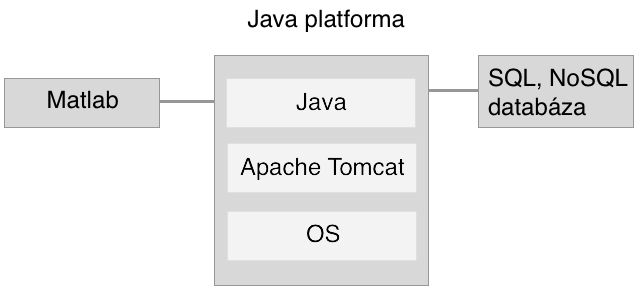
\includegraphics[scale=0.6]{img/platf/java-platform.png}
  \caption{Platforma Java.}
  \label{img-plat-java}
\end{figure}

\section{Návrh a implementácia StarkLab}
\indent Témou práce je navrhnúť a implementovať virtuálne laboratórium s využiťím JavaScriptu na strane servera. V tejto kapitole si ukážeme návrh celého virtuálneho laboratória s využitím technológií na jednotlivých komponentoch. O ich využití a konkrétnejšom popise sme si popísali viac v sekcii \ref{used-technologies}.

V zadaní sme sa dohodli o využití Node.js platformy ako náš server. Teda centrálny server (ďalej len StarkLab) - obrázok \ref{img-software-design}, ktorý spracováva dáta z Matlab workspace. 

\begin{figure}[H]
  \centering
  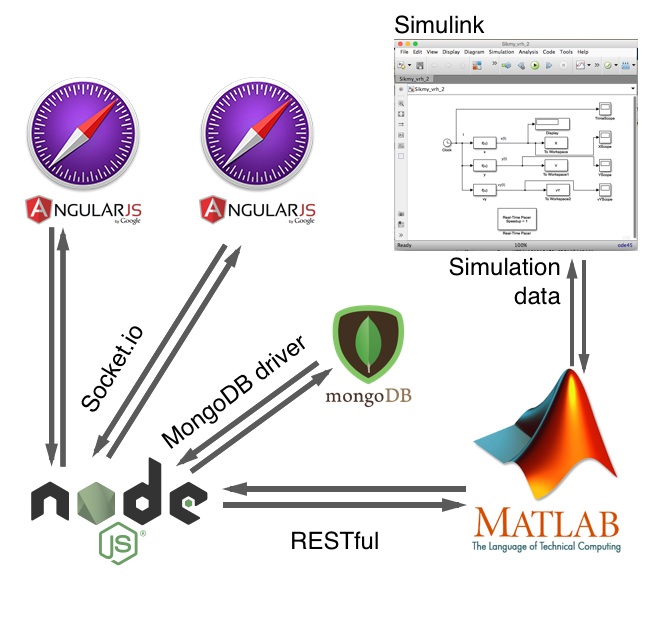
\includegraphics[scale=0.55]{img/StarkLab.png}
  \caption{Návrh komunikácie medzi komponentami VL.}
  \label{img-software-design}
\end{figure}

Do workspace Matlabu sa dáta získavajú v intervaloch zo Simulinku, v ktorom bola spustená referenčná schéma generujúca dáta. Zo začiatku nebolo isté či bude možné docieliť spustenie Simulinku v reálnom čase multiplatformovo. Našli sme riešenie Simulink Real-time priamo od Mathworks, ktorá toto umožnuje ale bohužial len pre operačný systém Windows. Lenže neskôr sme našli knižnicu \verb|tos_lib.mdl|, ktorá nám túto funkcionalitu umožňuje aj pod MAC OS X. Táto knižnica poskytuje množstvo blokových schém, z ktorej sme využili len blokovú schému real-time pacer. Tá slúži na spomalenie simulácie do soft real-time.

Na komunikáciu s workspace používame volanie RESTful služieb, ktoré podporuje aj Matlab R2015b \cite{matlab-restful}. Po spustení simulácie cez webového klienta užívateľom sa dáta začnú prenášať cez \verb|Socket.io| kanál. Tieto dáta budú zobrazené v grafoch vo webovom prehliadači a bude možné ich uchovať aj v databáze MongoDB pre neskoršie spracovanie.

\subsection{Referenčný model simulácie v Matlabe}
Funkčné softwarové riešenie síce bude mať možnosť spolupracovať s reálnymi zariadeniami, no pre jeho vývoj sme použili simuláciu dynamického systému šikmého vrhu, ktorá sa spúšta cez webové rozhranie a vykonáva v Simulinku.

Pre načítanie simulácie je potrebné spustiť dva súbory. Účel prvého je inicializácia premenných potrebných pre výpočet súradníc polohy bodu v šikmom vrhu. Podľa kódu na obrázku \ref{img-matlab-function} vidíme, že je potrebné zadať parametre pre spustenie a jej návratová hodnota nie je žiadna. Prvý z parametrov \verb|v0| predstavuje počiatočnú rýchlosť telesa v metroch za sekundu, akou bude vymrštené z bodu \textbf{(0,0)}. Druhý parameter \verb|alfa_deg| zase určuje, pod akým uhlom v stupňoch, bude teleso vymrštené. Posledný parameter \verb|userFromWeb| nie je potrebný k samotnej simulácií, ale hlavne pre identifikáciu užívateľa, ktorý spustil simuláciu. Vďaka tomu je možné mu priradiť výsledky simulácie pri neskoršom spracovaní z databázy.

\begin{figure}[H]
  \centering
  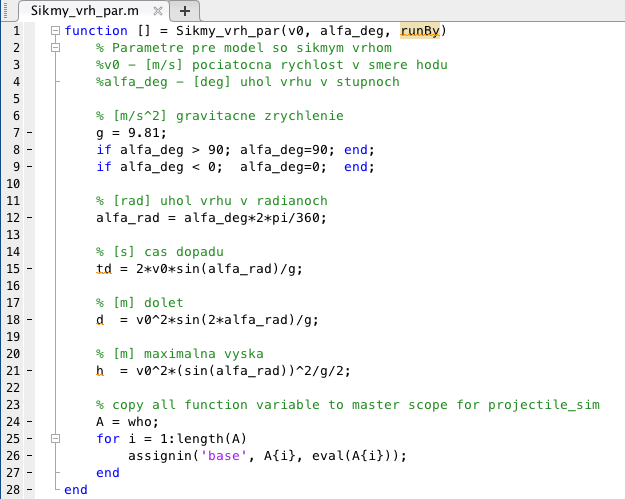
\includegraphics[scale=0.7]{img/code/matlab-function.png}
  \caption{Inicializačná funkcia šikmého vrhu v Matlabe.}
  \label{img-matlab-function}
\end{figure}

Keď sú parametre funkcie správne zadané a spustí sa telo funkcie, tak sa nastavia a vypočítajú hodnoty ako \verb|alfa_rad, td, d, h|, ktorých popis vidíme na obrázku a sú potrebné ako vstupné parametre do simulácie.

Posledná časť kódu od riadku č. 23 slúži pre prekopírovanie premenných do hlavného scope Matlabu, čiže workspace. Ak túto časť vynecháme, tak všetky hodnoty po skončení funkcie zaniknú, pretože sú tam lokálne premenné. Bolo by možné sa tomuto vyhnúť v prípade, že by sme nevolali funkciu \verb|Sikmy_vrh_par(80, 70, 'xstark')|, ale volali priamo len súbor, vďaka čomu by zostali všetky hodnoty v hlavnom workspace. Lenže pri tomto spôsobe riešenia by nebolo možné nastaviť inicializačné hodnoty ako parametre funkcie z webovej aplikácie, ale by museli byť natvrdo nastavené v kóde Matlabu.

Ako sme si už povedali, hodnoty sa po spustení úspešne uložia do Matlab workspace a to vidieť aj na obrázku \ref{matlab-function-workspace}. Tieto hodnoty boli vygenerované po zavolaní funkcie so špecifickými hodnotami parametrov \verb|Sikmy_vrh_par(80, 70, 'xstark')|.

\begin{figure}[H]
  \centering
  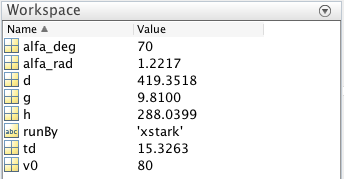
\includegraphics[scale=0.7]{img/code/matlab-function-workspace.png}
  \caption{Hodnoty v Matlab workspace po spustení funkcie.}
  \label{matlab-function-workspace}
\end{figure}

Druhý súbor, ktorý potrebujeme spustiť po tomto je obslužný kód, vďaka ktorému vieme zaslať údaje do Node.js. Kvôli jeho dĺžke a vlastnej implementácii ho nie je možné zobraziť celý, tak si popíšeme len kľúčové vlastnosti.

Pri inicializácií sa nastavi URL cesta pre Express.js API, na ktorú bude Matlab posielať dáta.
Model sa prednačíta pomocou funkcie \verb|load_system('Sikmy_vrh_2')|. Táto funkcia vyhľadá v aktuálnom priečinku súbor \verb|Sikmy_vrh_2.mdl| a nastaví ho ako aktuálny top-level model. Po nastavení je potrebné ešte simuláciu aj spustiť. Ovládanie simulácie sa robí pomocou príkazu \verb|set_param(model, 'SimulationCommand', 'Start')|, kde posledný parameter znamená spustenie simulácie.
Následne sa spustí \textbf{nekonečný while} cyklus, vďaka ktorému je možné zbierať údaje zo simulácie, až do stavu, kým nie je ukončená. 

Na začiatku cyklu sa volá \verb|set_param(model, 'SimulationCommand',| \\ \verb|'WriteDataLogs')| čo vlastne pristúpi k aktuálne najvyššie spustenej simulácií a snaží sa realtime zapisovať vypočítané hodnoty do Matlab workspace. Bez tohto príkazu by sa zapísali až po skončení simulácie.

Medzitým sa údaje upravujú na potrebný formát a pred odoslaním na REST API je vhodné ho zabaliť do JSON štruktúry. Tú vieme vytvoriť pomocou knižnice \verb|jsonlab| v aktuálnej verzii 1.2.
Pomocou sekvencie týchto dvoch príkazov vytvoríme požadovaný JSON formát a odošleme ho na Express.js API. Vytvorenie JSON \verb|json = savejson('result',| \\ \verb|struct('user', userFromWeb, 'status', 'running', 'data', struct('time',| \\ \verb|timeFinal, 'vy', vyFinal, 'y', yFinal, 'x',xFinal)))| a jeho následné zaslanie do služby \verb|response = webwrite(url, json, options)|.

Pomocou príkazu \verb|get_param(model, 'SimulationStatus')| vieme získať aktuálny stav simulácie. V prípade, že simulácia stále beží tak získame výstup \verb|"running"| inak je ukočená a vráti reťazec \verb|"stopped"|. Hneď ako dostaneme status \verb|"stopped"| tak ukončíme cyklus pomocou \verb|break| a vieme, že všetky dáta su prenesené do Node.js.

\subsection{Diagramy}
Pred tvorbou rôznych softvérových systémov zväčša nezačneme hneď programovať, ale najprv si zadefinujeme požiadavky, ktoré by mal spĺňať. Následne na základe požiadaviek vytvoríme diagramy, podľa ktorých sa neskôr budeme riadiť pri tvorbe software. Niektoré nám hovoria o správaní len vo všeobecnosti, čo by sa mohlo dať v systéme robiť, ako napr. \textbf{prípady použitia}. Potom existuje aj \textbf{diagram tried}, ktorý slúži na vizualizáciu jednotlivých tried, ktoré sa tvoria v objektovo orientovaných jazykoch. Diagram tried v našom prípade nie je možné vytvoriť, pretože JavaScript nie je klasický objektovo orientovaný jazyk. Ale zase môžeme využiť \textbf{sekvenčné diagramy}, pretože tie nám hovoria o interakcií medzi jednotlivými komponentami, prípadne časťami kódu.

\subsubsection{Prípad použitia}
Diagram prípadov použitia sa používa k popisu chovania systému z hľadiska užívateľa a zachytáva, ktoré typy užívateľov so systémom pracujú a aké činnosti v rámci systému vykonávajú \cite{uml-usecase}.

Na obrázku \ref{img-use-case} vidíme možnosti používania systému na diagrame prípadov použitia. V systéme vystupuje len jeden typ používateľa a musí to byť člen STUBA LDAP. Bez prihlásenia sú jeho možnosti obmedzené a nemôže nič pozerať ani vykonávať. Po prihlásení môže vykonať dve úlohy. Zobrazenie už existujúcich simulácií alebo vybrať simuláciu, ktorú chce spustiť s počiatočnými parametrami ak sú potrebné.

\begin{figure}[H]
  \centering
  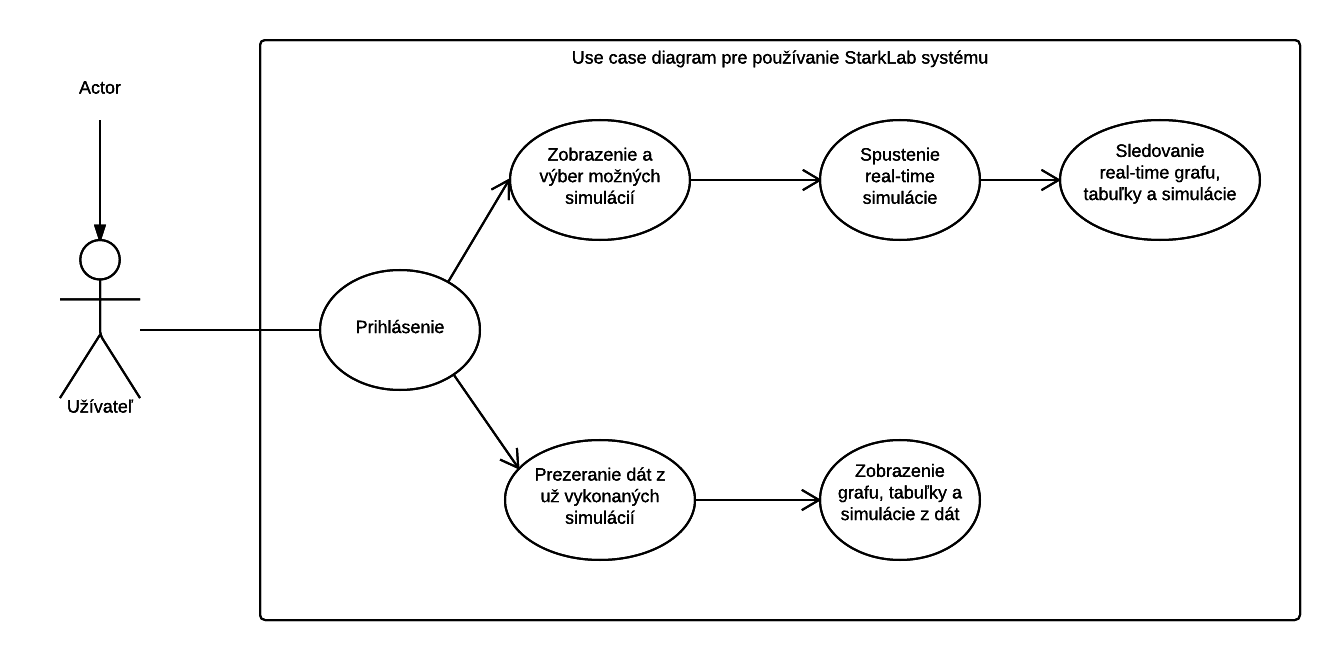
\includegraphics[scale=0.75]{img/diagrams/use-case.png}
  \caption{Diagram prípadu použitia na prácu zo systémom.}
  \label{img-use-case}
\end{figure}

\subsubsection{Diagram tried}
Síce sme hovorili o tom, že klasický diagram tried nie je možné vytvoriť pre JavaScript aplikáciu, ale našli sme knižnicu \verb|wavi| (https://www.npmjs.com/package/wavi), ktorá dokáže vygenerovať takýto diagram. Síce to nie je prehľadné ako pri klasickom diagrame, ale je vhodné ho vygenerovať už len pre to, aby mal programátor prehľad o základnej štruktúre aplikácie - obrázok \ref{img-class-diagram}.

\begin{figure}[H]
  \centering
  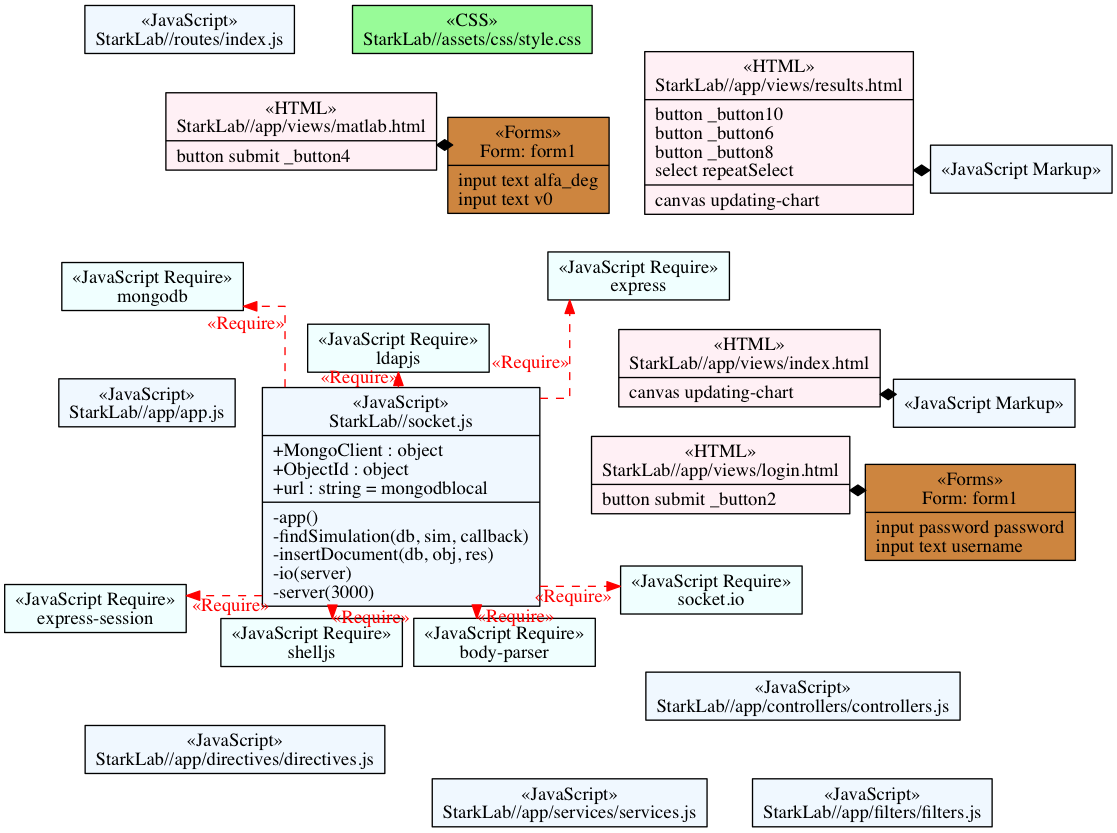
\includegraphics[scale=0.34]{img/diagrams/class.png}
  \caption{Diagram štruktúry systému.}
  \label{img-class-diagram}
\end{figure}

\newpage
\subsubsection{Sekvenčný diagram}\label{diagram-sequence-section}
Sekvenčný diagram patrí medzi najviac používané diagramy pre zobrazenie interakcií. Zachytáva priebeh spracovania v systéme v podobe posielania správ.\\


\noindent \textbf{Prihlásenie do LDAP}

Na obrázku \ref{img-sequence-ldap-login} je spôsob prihlásenie pomocou mena a hesla do LDAP systému.

\begin{figure}[H]
  \centering
  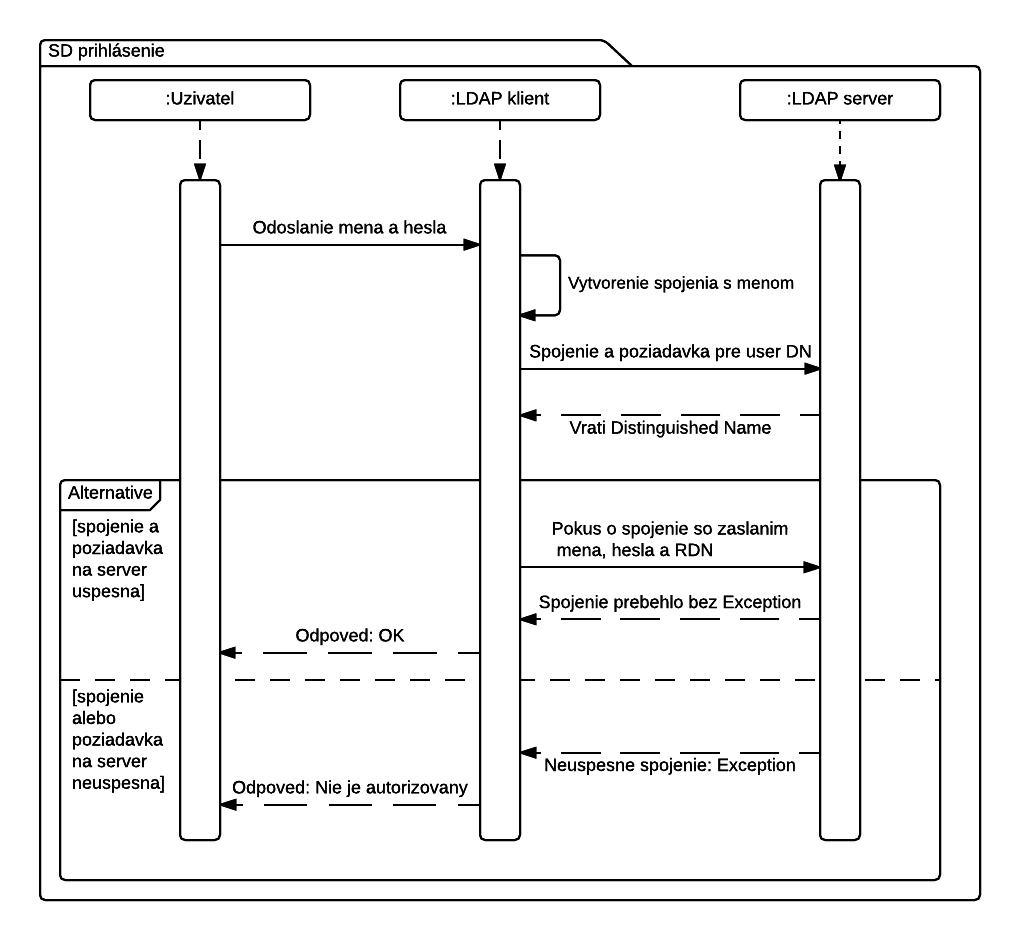
\includegraphics[scale=0.8]{img/diagrams/sequence-ldap.png}
  \caption{Sekvenčný diagram pre prihlásenie pomocou LDAP.}
  \label{img-sequence-ldap-login}
\end{figure}

Nižšie si popíšeme kód z obrázka \ref{img-sequence-ldap-login-js}, ktorým to bolo implementované v JavaScripte. Toto je len časť kódu, ktorá sa určená pre prihlásenie do systému. Na začiatku súboru je volaná požadovaná knižnica pre prácu s LDAP ako \verb|var ldap = require("ldapjs")|.

Keď užívateľ príjde na stránku a vyplní prihlasovacie meno a heslo do stuba ldap, tak formulár ho presmeruje na \verb|/login|, kde už sa postaral o routovanie Express.js. Z \verb|request| parametra získame username - \verb|req.body.username| a password - \verb|req.body.password|, ktoré boli vyplnené pred odoslaním formulára. Čiže ak sú oba vyplnené dostaneme sa do vnútra podmienky, kde sa vytvorí spojenie na linku \verb|ldap://ldap.stuba.sk|, a zašle RDN reťazec v tvare \verb|"uid=xstark", ou=People, DC=stuba, DC=sk"|.

V momente, keď je zostavený reťazec a máme získané heslo užívateľa, tak zavoláme ldap funkciu \verb|bind| s parametrami RDN a heslom. V prípade ak overovanie prebehlo bez chyby, tak autorizácia prebehla úspešne. Potom vytvoríme \verb|session| a \verb|cookie| pre užívateľa a presmerujeme ho na stránku, kde už môže vidieť simulácie.

\begin{figure}[H]
  \centering
  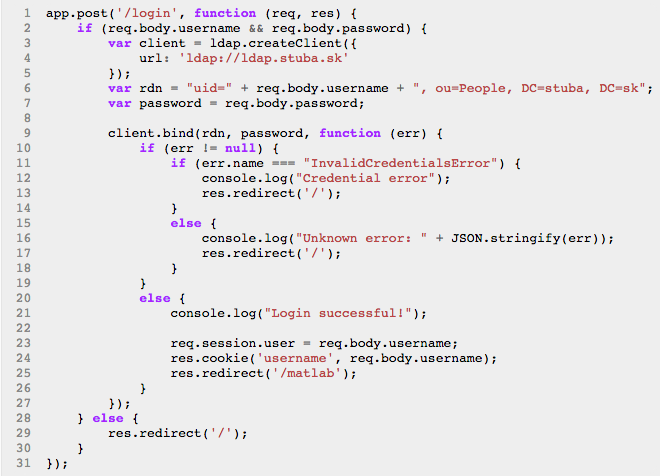
\includegraphics[scale=0.68]{img/code/ldap-login.png}
  \caption{Prihlásenie do aplikácie pomocou LDAP v JavaScripte.}
  \label{img-sequence-ldap-login-js}
\end{figure}

\noindent \textbf{Komunikácia komponentov v systéme}

Medzi jednotlivými komponentami systému prebieha komunikácia. Síce v každej časti prebieha inak, ale ich spoločný menovateľ je komunikácia založená na HTTP protokole.

Na obrázku \ref{img-sequence-realtime} vidíme, že komunikácia začína od webového klienta v prehliadači. Užívateľ zadá parametre simulácie a tie budú zaslané do StarkLab. Ten následne spustí Matlab na aktuálnom operačnom systéme s potrebnými súbormi simulácie a ich parametrami. Medzitým užívateľ čaká kým sa na pozadí spustí Matlab. Hneď po spustení začne vykonávať simuláciu a posielať údaje do StarkLab, ktorý ich pošle priamo webovému klientovi, odkiaľ bola simulácia spustená. Každé prijatie údajov sa prejaví zapísaním do grafu, animácie a tabuľky vo webovom rozhraní. Táto sekvencia sa opakuje pokiaľ platí podmienka \verb|SimulationStatus == "running"|. Po zastavení simulácie klient zašle požiadavku na zapísanie kompletných dát cez StarkLab priamo do dokumentovej databáze MongoDB.

\begin{figure}[H]
  \centering
  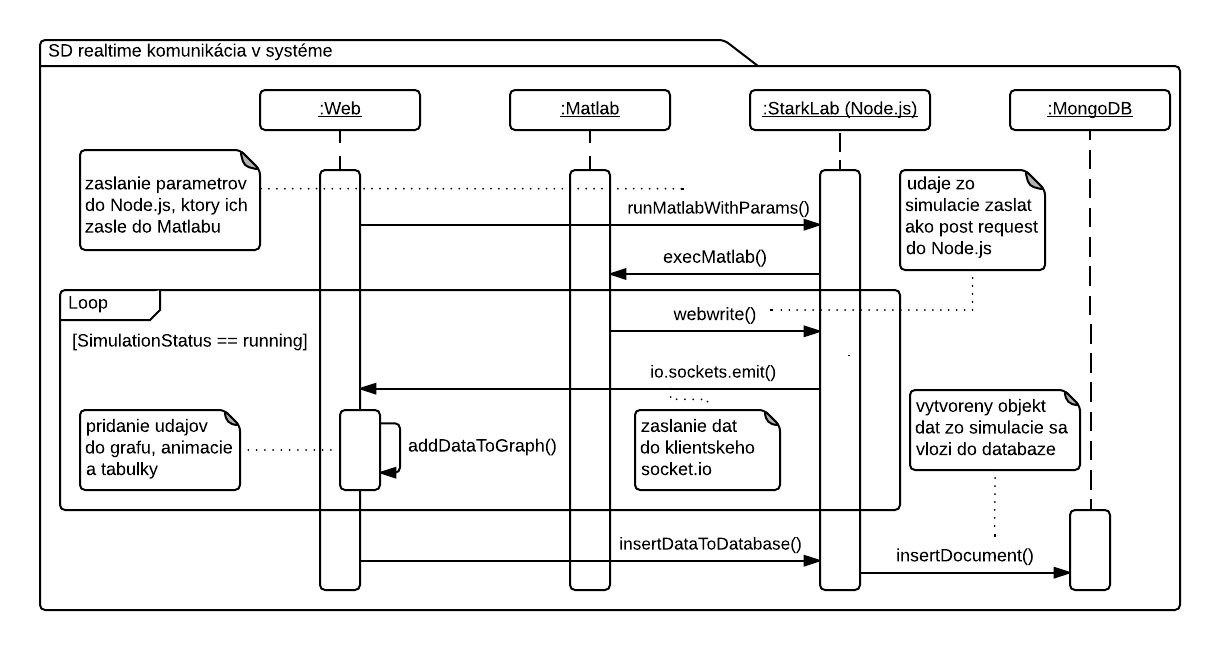
\includegraphics[scale=0.38]{img/diagrams/sequence-realtime-communication.png}
  \caption{Komunikácia medzi jednotlivými komponentami systému.}
  \label{img-sequence-realtime}
\end{figure}

\subsection{Databázový model MongoDB}
V našom zadaní sme nepoužívali štandardnú SQL databázu, čiže nie je možné využiť bežné modelovanie cez ERD diagramy. Ako už vieme MongoDB neukladá dáta ako tabuľky, ale JSON dokumenty. Keďže sa jednalo o jednoduchý model šikmého vrhu, tak v tomto prípade nebude model zložitý. V tejto časti si ukážeme, do akého objektu ho v JavaScripte ukladáme a potom konkrétny príklad záznamu z databázy.

\begin{figure}[H]
  \centering
  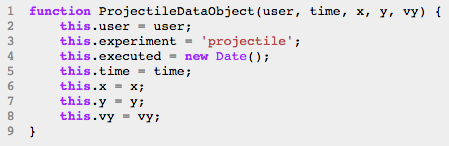
\includegraphics[scale=0.8]{img/code/javascript-projectile-model.png}
  \caption{Model objektu v JavaScripte, pre vytvorenie záznamu v MongoDB.}
  \label{img-js-projectile-model}
\end{figure}

Ako vidíme v JavaScripte nepotrebujeme špecifikovať nejaké štandardné typy. Hodnoty premenných \verb|user, experiment| budú vždy typu String, \verb|executed| je typu Date v štandardizovanom formáte ISO-8601, ktorého formát pre zobrazenie je YYYY-MM-DDTHH:mm:ss.sssZ. Hodnoty premenných \verb|time, x, y, vy| sú závislé od simulácie a každá z nich je pole čísiel.

Obrázok \ref{img-mongo-record} je záznam z MongoDB, kde konkrétne hodnoty time, x, y, vy nie sú zobrazené, pretože simulácia vygenerovala až 788 hodnôt.

\begin{figure}[H]
  \centering
  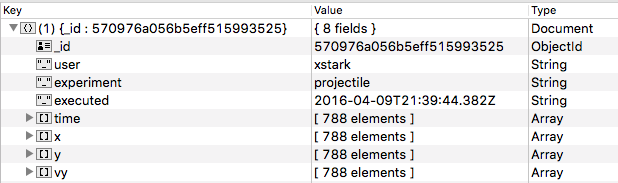
\includegraphics[scale=0.7]{img/code/mongodb-record.png}
  \caption{Príklad záznamu simulácie v MongoDB.}
  \label{img-mongo-record}
\end{figure}

%\section{Testovanie}

\subsection{Node.js s frameworkom Express.js}
Hlavná časť tejto práce je sústredená na komunikáciu medzi Matlabom a Node.js, resp Express.js. Využívame ich posledné verzie Node.js verzie 6.1.0 a Express.js verzie 4.13.4. Je to vlastne len framework umožňujúci jednoduchšiu tvorbu REST služieb. Na začiatok si povieme, čo sme použili ako \verb|middleware|. Ako už bolo napísané je to funkcia, ktorá má prístup do request a response objektu. Použili sme \verb|body-parser|, ktorý nám umožnil spracovávať telo POST požiadavky, ktorá bola odoslaná z Matlabu. Každý middleware, ktorý chceme použiť je potrebné aj aktivovať v kóde \verb|app.use(bodyParser.json({limit: '2mb'}))|. Po viacerých testoch som zistil, že základný limit je nastavený na 1MB, kde sa vyskytoval problém s prijatím POST requestu, keď boli dáta veľmi veľké.

\subsubsection{Vlastný middleware prihlasovania}
V aktuálnom softwarovom riešení nebolo potrebné vytvoriť prihlasovanie, pretože neskôr bude integrované do \textbf{LMS Moodle}, ktorý prihlasovanie rieši vlastným spôsobom. Ale pre ukážku možností frameworku Express.js sme implementovali middleware \verb|express-session|, vďaka ktorému môžme vytvoriť reláciu pre úspešne autorizovaného užívateľa. 

Pri implementácii prihlasovania cez session sme zistili, že v každom smerovaní, bolo potrebné kontrolovať na začiatku kódu, či tam pristupuje prihlásený používateľ alebo požiadavka z Matlab služby. Pri väčšom projekte, prípadne viacerých smerovaní by to začalo byť neefektívne a neprehľadné. 

Vytvorili sme vlastný middleware na obrázku \ref{img-code-express-middleware}, ktorý slúži na overenie prihláseného užívateľa pri každom prístupe na akékoľvek smerovanie.

\begin{figure}[H]
  \centering
  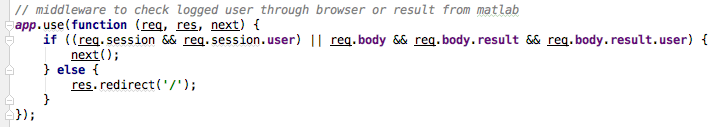
\includegraphics[scale=0.6]{img/code/express-middleware.png}
  \caption{Middleware kód v Express.js na kontrolu prihlásenia.}
  \label{img-code-express-middleware}
\end{figure}

Volanie \verb|app.use| nám zabezpečí, že sa táto funkcia zaregistruje ako middleware a bude volaná pri každom requeste. Prvá časť podmienky overuje, či prichádzame z webového prehliadača a je nastavená session. Kedže Matlabu nevieme nastaviť session, pretože tá sa ukladá len na webserveri, tak sme to vyriešili iným spôsobom. V prichádzajúcom tele POST requestu od Matlabu je objekt \verb|result|, kde sú uložené simulované dáta. Priradili sme mu ďalšiu vlastnosť \verb|user|, ktorá keď je nastavená, tak vieme, že požiadavka prichádza z Matlabu a povolíme jej prístup. V prípade splnenej aspoň jednej podmienky sa zavolá callback \verb|next()|, čo vyvolá ďalší zaregistrovaný middleware, alebo už smerovanie, na ktoré sme posielali požiadavku.
Ak nie je splnená ani jedna z dvoch podmienok, tak server nás presmeruje na hlavnú stránku, kde je znovu požadované prihlásenie.


\subsubsection{Spustenie Matlabu z príkazového riadku}
Zo začiatku nebolo isté ako budeme spúšťať simuláciu, pretože sme nevedeli, či Node.js umožuje vykonávať príkazy nad operačným systémom, resp. spúšťať programy. Vtedy sme komunikáciu riešili takým spôsobom, že Matlab sa otvoril ručne a v ňom sme spustili potrebné inicializačné súbory a následne samotnú simulácia. Takéto riešenie nie je postačujúce z hladiska automatizácie a samostatnosti.

Potom sme zistili, že Node.js má možnosti na spustenie akéhokoľvek softvéru, ktorý je možné spustiť aj cez terminál. Pre zjednodušenie práce bol využitý modul \verb|shelljs|, ktorý takúto možnost poskytuje.

Na obrázku \ref{img-express-shelljs} je funkcionalita, ktorá sa vykoná po prístupe na route /matlab/run. Táto časť sa volá po odoslaní formuláru s parametrami počiatočnej rýchlosti a uhlu z webového prehliadača.

\begin{figure}[H]
  \centering
  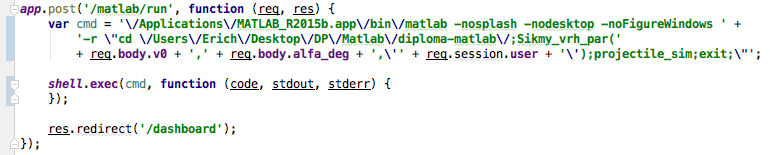
\includegraphics[scale=0.6]{img/code/express-shelljs.png}
  \caption{Spustenie príkazu v OS pomocou shelljs modulu.}
  \label{img-express-shelljs}
\end{figure}

Vstupný príkaz vo forme reťazca, ktorý chceme vykonať, musí mať správne zadanú cestu k Matlabu na súborovom systéme. Matlab spúštame v termináli s parametrami, ktoré umožnujú spustenie bez nepotrebných častí pre našu simuláciu \cite{matlab-macos}. Ako napr. nepotrebujeme vidieť výsledky v okne, alebo animáciu Matlabu pri spustení. Pomocou parametra \verb|-r| vieme volať príkazy v príkazovom riadku Matlabu, napr. špecifikovať cestu, kde sa nachádza naša simulácia a potrebné súbory. Následne zavoláme funkciu \verb|Sikmy_vrh_par()|, s ktorou sa pošlú parametre počiatočnej rýchlosti, uhla a zároveň meno prihláseného používateľa. Po vykonaní tejto funkcie sa spustí súbor simulácie \verb|projectile_sim|. Po jej skončení zatvoríme Matlab pomocou príkazu \verb|exit|.

Po zostrojení tohto reťazca ako parametra funkcie \verb|exec()| a jeho spustení sa čaká na vykonávanie Matlabu. Medzitým nás server presmeruje na stránku /dashboard kde sa čaká na údaje zo simulácie. V momente načítania simulácie so vstupnými parametrami sa dáta zobrazia realtime vo webovom prehliadači.

\subsubsection{Práca s dátami simulácie}
Po načítaní simulácie je Matlab pripravený poslať výsledky na smerovanie, ktoré vidíme na obrázku \ref{img-express-socketio}. 

\begin{figure}[H]
  \centering
  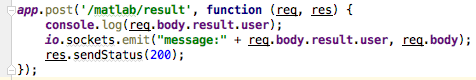
\includegraphics[scale=0.7]{img/code/express-socketio.png}
  \caption{Prijímanie a zasielanie dát pomocou Socket.io do prehliadača.}
  \label{img-express-socketio}
\end{figure}

Výsledky z Matlabu máme uložené v tele každého requestu, ktorý prijde. Následne môžeme k nim prístupiť pomocou \verb|req.body|. Pôvodne \textbf{Socket.io} odosielal údaje len na kanál "message". V takom prípade by sme ale nevedeli identifikovať, ku ktorému uživateľovi sa majú posielať údaje. Po implementácii session sme zvážili, že by ich bolo lepšie posielať priamo na adresu "message:xstark", teda s menom prihláseného užívateľa. Vždy po prijatí je potrebné odoslať status kód 200, čo v HTTP znamená OK po úspešnom prijatí dát.


\subsubsection{Zápis dát do MongoDB}
Po prijatí a zobrazovaní dát nasleduje spracovanie. Ich spracovanie sa vykonáva na úrovni Express.js za pomoci MongoDB ovládača.

Na začiatku je potrebné najprv zavolať modul a následne jeho klientskú časť cez \verb|var MongoClient = require('mongodb').MongoClient|. Potom nasleduje definovanie URL, na ktorej máme spustenú databázu \verb|mongodb://localhost:27017/test|.

Najprv si ukážeme funkcie, ktoré vykonávajú svoju úlohu, až potom ich použitie. Prvá z nich je vloženie dokumentu do databázy na obrázku \ref{img-express-mongo-insert}. Táto funkcia slúžiaca na vytvorenie jedného záznamu sa pokúsi vložiť \verb|obj| do kolekcie \textbf{projectile}, kde sú vlastne naše kompletné záznamy zo simulácií. Po úspešnom vložení zatvorí prihlásenie na databázu a vráti HTTP status kód 200.

\begin{figure}[H]
  \centering
  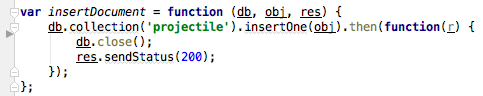
\includegraphics[scale=0.7]{img/code/express-mongo-insert.png}
  \caption{Vloženie záznamu do MongoDB pomocou JavaScriptu.}
  \label{img-express-mongo-insert}
\end{figure}

Druhá funkcia, ktorú využívame na prácu s databázou je na obrázku \ref{img-express-mongodb-find}. 
Slúži na vyhladanie záznamu v závislosti od parametrov. Jednu funkciu vieme využiť na viacero účelov. V prípade ak zadáme parameter funkcie \verb|sim|, tak v podmienke sa skontroluje, či je dostupná vlastnosť \verb|id|. Ak áno, tak vyhľadanie v databáze prebehne na základe parametrov užívateľského mena a konkretného id simulácie, čo nám vyhľadá iba jeden záznam, ak existuje. V opačnom prípade vyhľadá všetky záznamy simulácií pre daného užívateľa. Táto funkcionalita sa využíva pri zobrazení všetkých záznamov u klienta.

\begin{figure}[H]
  \centering
  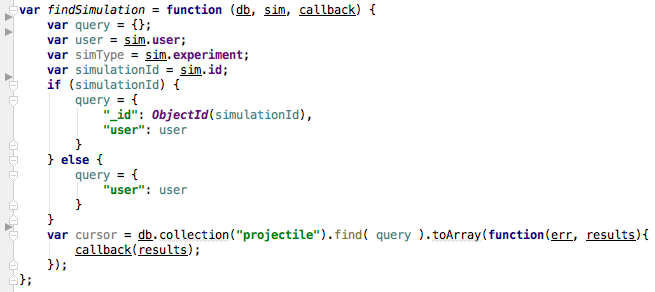
\includegraphics[scale=0.65]{img/code/express-mongodb-find.png}
  \caption{Vyhľadanie záznamu v MongoDB pomocou JavaScriptu.}
  \label{img-express-mongodb-find}
\end{figure}

Po ukážke implementácií funkcií, ktoré vykonávajú zápis/čítanie si ukážeme ich volanie. Na obrázku \ref{img-express-mongodb-insert2} je vloženie záznamu po prístupe na smerovanie /mongo/insert/one.
Pre vykonanie nejakej operácie nad databázou musíme vytvoriť spojenie medzi klientom a MongoDB. Slúži na to funkcia \verb|connect(url, callback)|, ktorej prvý parameter je URL, kde sa nachádza DB a druhý je callback, kde sa vracajú údaje.

\begin{figure}[H]
  \centering
  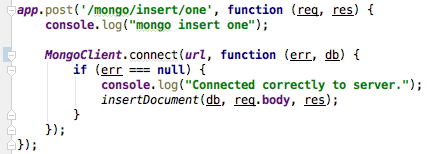
\includegraphics[scale=0.7]{img/code/express-mongo-insert2.png}
  \caption{Volanie vloženia záznamu do MongoDB.}
  \label{img-express-mongodb-insert2}
\end{figure}

Pre vyhľadanie záznamu na obrázku \ref{img-express-mongodb-find2} sa s pripojením nič nemení.
Rozdiel je iba vo využití volania smerovania. Dvojbodka pred názvom \verb|:user| znamená, že tento parameter môže byť v URL dynamický. Otáznik pri parametri ako pri \verb|:id?| znamená, že tento nie je povinný, a URL može byť volaná aj bez neho. Ak sa teda v URL nachádzajú parametre, pristupujeme k nim pomocou poľa \verb|req.params|.

\begin{figure}[H]
  \centering
  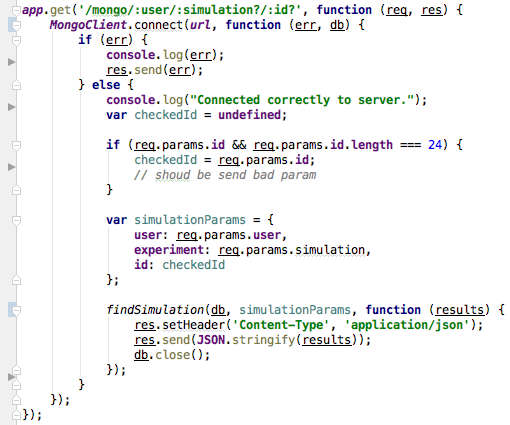
\includegraphics[scale=0.7]{img/code/express-mongodb-find2.png}
  \caption{Volanie vyhľadania záznamu v MongoDB.}
  \label{img-express-mongodb-find2}
\end{figure}
 
\subsection{Webový klient s frameworkom Angular.js}
Na klientskú časť práce sme využili JavaScriptový framework Angular.js v poslednej stabilnej verzii 1.5.5. Úlohou webového klienta bolo overiť funkčnosť vytvoreného prostredia, ktorý posiela simulované dáta. Funkčnosť sme overili a popíšeme si konkrétne obrazovky.

\begin{figure}[H]
  \centering
  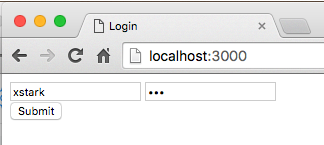
\includegraphics[scale=0.45]{img/code/angular-login.png}
  \caption{Prihlásenie do LDAP pomocou STUBA údajov.}
  \label{img-angular-login}
\end{figure}

Ako to funguje na pozadí sme si popísali v sekcii \ref{diagram-sequence-section}, kde sa pojednávajú sekvenčné diagramy, konkrétne prihlásenie do LDAP.
Po prihlásení sa zobrazí stránka vyhradená pre zadanie parametrov šikmého vrhu: počiatočnej rýchlosti v0 a uhlu vystrelenia alfa\_deg. Rovnako sú tu popísané aj základné informácie o simulácii a jeho vzorcov.

Po zadaní rýchlosti \textbf{v0=40} a \textbf{alfa\_deg=60} sme presmerovaní na stránku /matlab.

\begin{figure}[H]
  \centering
  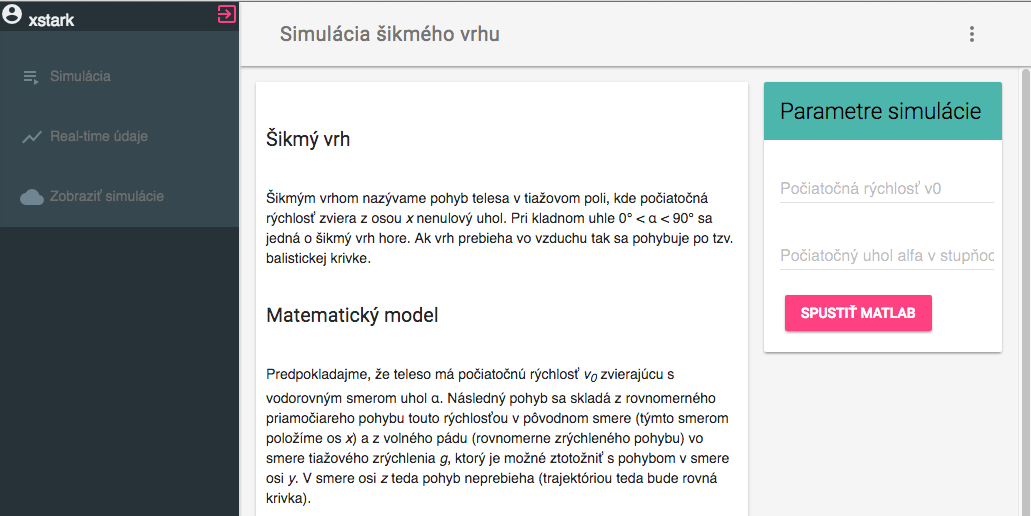
\includegraphics[scale=0.42]{img/code/angular-simulation-param.png}
  \caption{Parametre simulácie - počiatočná rýchlosť a uhol v stupňoch.}
  \label{img-angular-params}
\end{figure}

\subsubsection{Grafy s Chart.js}
Pre vizualiáziu prichádzajúcich dát používame knižnicu na grafy \verb|Chart.js|, ktorá je vytvorená pomocou HTML canvas. Využívame poslednú verziu jednotkovej rady 1.1.1. \verb|<script src="/node_modules/chart.js/Chart.min.js"></script>| je zápis volania v HTML hlavičke. Ako si môžeme všimnúť, tak nie je závislá od žiadnej online CDN služby, ale jej inštalácia prebehla lokálne pomocou NPM.

Vyvorili sme Angular.js directívu \verb|uiGraph|, ktorá slúži pre vytvorenie grafu na potrebnom mieste. Ako template obsahuje \verb|<canvas id="updating-chart" width="600"| \\ \verb|height="300"></canvas>|. Na obrázku \ref{img-angular-chartjs-canvas} vidíme vytvorenie grafu a nastavenie hodnôt. Táto časť kódu sa nachádza v postLink funkcii directívy.

Na začiatku je potrebné získať element z DOM, získať kontext canvasu a vytvoriť objekt \verb|startingData| s nastaveniami pre inicializačné dáta. 
Následne je potrebné vytvoriť inštanciu grafu, kde sa ako parameter grafu použije kontext canvasu. Potom sa volá funcia čiarového grafu, ktorý tam chceme využiť. Tá zase vyžaduje ako vstupný parameter inicializačné dáta. Túto directívu zavoláme v HTML ako \verb|<ui-graph></ui-graph>| element.\\

Ak by sme chceli rozšíriť graf, resp. ak by bolo rozumné súčasne vykreslovať viacero závislých veličín, tak je možné zadefinovať ďalší dataset.

\begin{figure}[H]
  \centering
  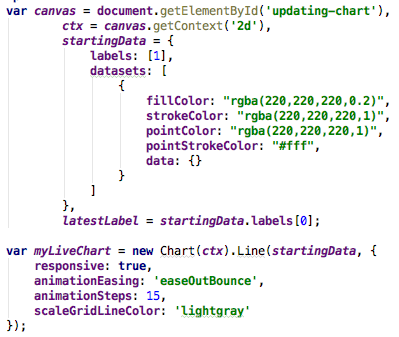
\includegraphics[scale=0.6]{img/code/angular-chartjs-code.png}
  \caption{Inicializácia hodnôt pre Chart.js.}
  \label{img-angular-chartjs-canvas}
\end{figure}

Po presmerovaní na stránku /dashboard pri sekcii real-time treba počkať, kým sa spustí Matlab so simuláciou a následne sa začnú vkladať realtime dáta do webového prehliadača. Táto časť by mohla byť zrýchlená tým, že sa Matlab bude nachádzať na výkonnom serveri. Na obrázku \ref{img-angular-chartjs} je využitá knižnica Chart.js pre zobrazenie grafov.

\begin{figure}[H]
  \centering
  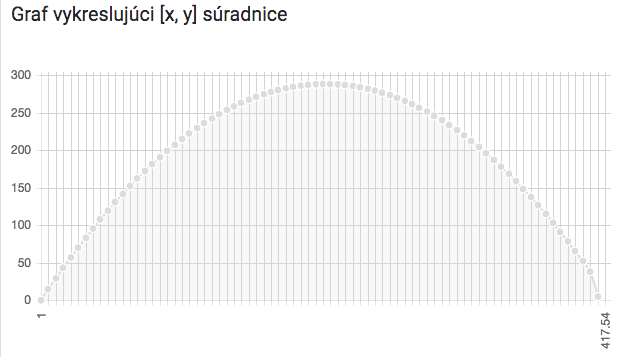
\includegraphics[scale=0.4]{img/code/angular-chartjs.png}
  \caption{Graf vykreslujúci závislosti [x, y] v šikmom vrhu.}
  \label{img-angular-chartjs}
\end{figure}

\subsubsection{Animácia pomocou html canvas}\label{section-canvas}
Vykreslené dáta na obrázku \ref{img-angular-canvas} sú zhodné s dátami na grafe, len je to spôsobom animácie guličky. Táto animácia bola vytvorená pomocou html canvas technológie.

\begin{figure}[H]
  \centering
  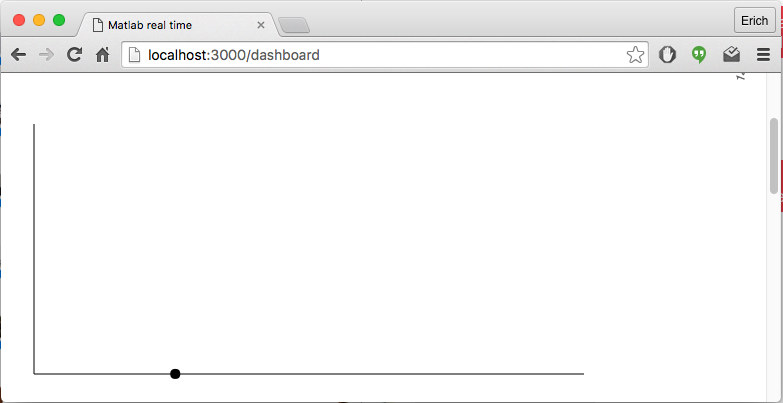
\includegraphics[scale=0.5]{img/code/angular-canvas.png}
  \caption{Animácia vykreslujúca závislosti [x, y] v šikmom vrhu.}
  \label{img-angular-canvas}
\end{figure}

\subsubsection{Tabuľka dát}
Ako posledná časť sledovania dát je tabulka, ktorej údaje sa vkladajú do zoznamu rovnako realtime ako aj pri grafe a animácii pred ním.

\begin{figure}[H]
  \centering
  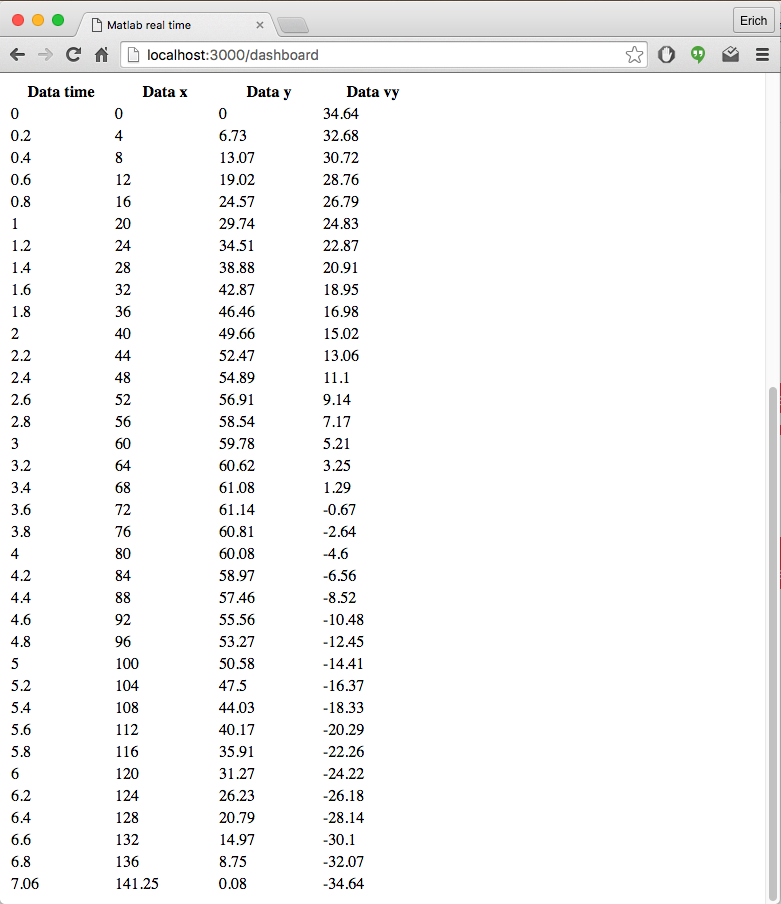
\includegraphics[scale=0.5]{img/code/angular-table.png}
  \caption{Tabuľka dát času, x, y a smer rýchlosti vy.}
  \label{img-angular-table}
\end{figure}


\subsubsection{Zobrazenie existujúcich simulácií}
V tomto systéme nejde len o real-time vykreslenie dát, ale aj o neskoršie zobrazenie a spracovanie. Po prejdení na stránku zo simuláciami, vidíme všetky záznamy simulácií pre aktuálne prihlaseného užívateľa - obrázok \ref{img-angular-results-projectile}.

\begin{figure}[H]
  \centering
  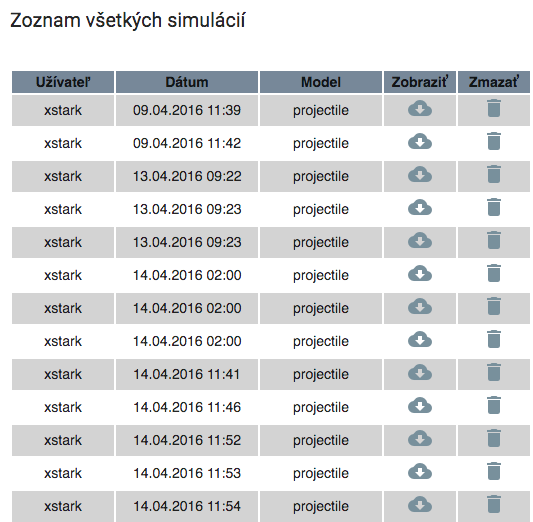
\includegraphics[scale=0.5]{img/code/angular-results-projectile.png}
  \caption{Zoznam uložených simulácií pre prihláseného užívateľa.}
  \label{img-angular-results-projectile}
\end{figure}

Pri zobrazení simulácie z databázy je možné mu nastaviť vzorkovanie, teda po koľkých dátach sa vykreslí graf - obrázok \ref{img-angular-fulldata-graph}. Ako vidíme, je možné využiť dve tlačidlá: jedno na okamžité vykreslenie a druhé pre pomalé vykreslenie, kde berieme do úvahy celkový čas simulácie.

\begin{figure}[H]
  \centering
  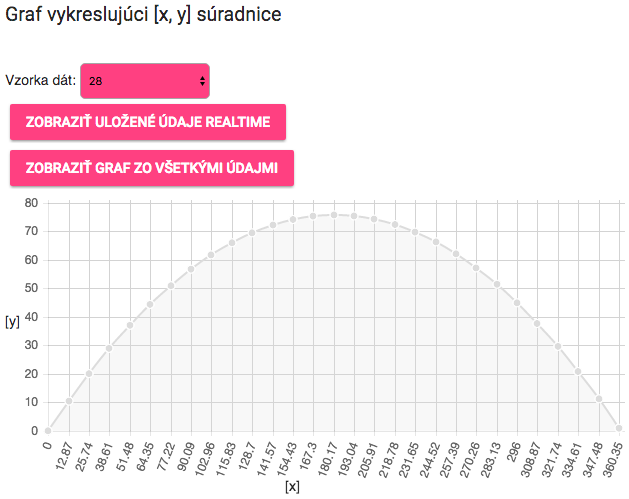
\includegraphics[scale=0.5]{img/code/angular-fulldata-graph.png}
  \caption{Graf pre vybranú vzorku dát.}
  \label{img-angular-fulldata-graph}
\end{figure}

Posledný obrázok \ref{img-angular-fulldata-animation} je o vykreslení animácie z databázy. Berie do úvahy nastavené vzorkovanie dát a čas vykreslenia.

\begin{figure}[H]
  \centering
  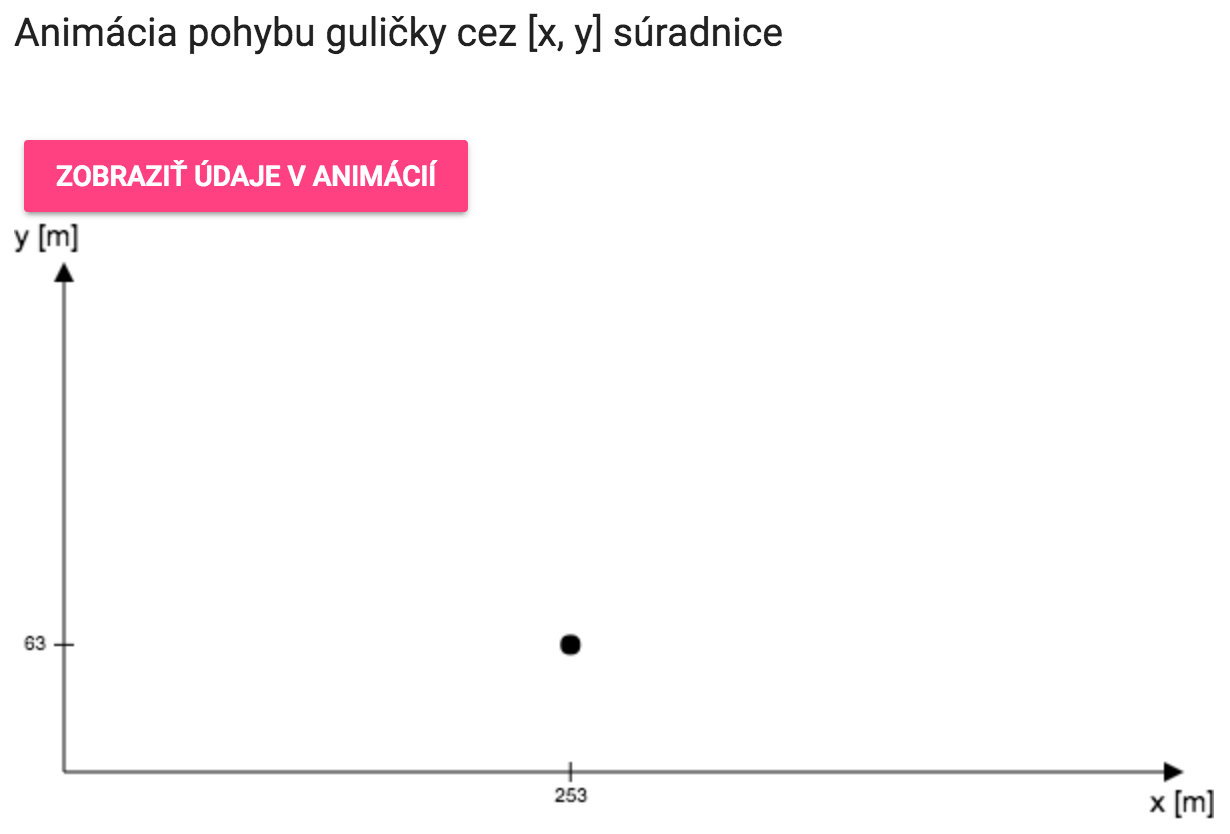
\includegraphics[scale=0.5]{img/code/angular-fulldata-animation.png}
  \caption{Animácia pre vybranú vzorku dát.}
  \label{img-angular-fulldata-animation}
\end{figure}

Na webovej stránke sa ešte pod animáciou nachádza rovnaká tabuľka ako v obrázku \ref{img-angular-table} s rozdielom, že v tejto tabuľke sú kompletné údaje a je možné ich exportovať do \verb|CSV| formátu.


%\section{Inštalácia vytvoreného riešenia}
%asi lepsie do prilohy
